\documentclass[UTF8,12pt]{ctexart}

\usepackage[a4paper,top=2.4cm,bottom=2.4cm,left=2.7cm,right=2.7cm]{geometry}
\usepackage{amsmath,amssymb,bm}
\usepackage{booktabs,longtable,tabularx,array,multirow}
\usepackage{graphicx,float,subcaption}
\usepackage{xcolor}
\usepackage{enumitem}
\usepackage{listings}
\usepackage{fancyhdr}
\usepackage{hyperref}
\usepackage{setspace}
\usepackage{caption}
\usepackage{titlesec}

\definecolor{navy}{HTML}{17365D}
\definecolor{lightblue}{HTML}{DCE6F1}
\definecolor{linegray}{HTML}{D9D9D9}
\definecolor{placeholder}{HTML}{6B7280}
\definecolor{codebg}{HTML}{F5F7FA}
\definecolor{codegreen}{HTML}{2E7D32}

\hypersetup{
  colorlinks=true,
  linkcolor=navy,
  citecolor=navy,
  urlcolor=navy,
  pdftitle={图像异常检测论文复现报告初稿},
  pdfauthor={待填写}
}

\setlength{\parindent}{2em}
\setlength{\parskip}{0.35em}
\linespread{1.35}
\setlist[itemize]{leftmargin=2em,itemsep=0.25em}
\setlist[enumerate]{leftmargin=2em,itemsep=0.25em}
\captionsetup{font=small,labelsep=quad}

\titleformat{\section}{\heiti\zihao{3}\bfseries\color{black}}{\thesection}{0.8em}{}
\titleformat{\subsection}{\heiti\zihao{4}\bfseries\color{black}}{\thesubsection}{1em}{}
\titleformat{\subsubsection}{\heiti\zihao{-4}\bfseries\color{black}}{\thesubsubsection}{1em}{}
\titlespacing*{\section}{0pt}{1.8em}{0.8em}
\titlespacing*{\subsection}{0pt}{1.3em}{0.5em}

\pagestyle{fancy}
\fancyhf{}
\setlength{\headheight}{14pt}
\fancyhead[L]{\small 图像异常检测论文复现报告}
\fancyhead[R]{\small 论文复现报告初稿}
\fancyfoot[C]{\thepage}
\renewcommand{\headrulewidth}{0.4pt}
\renewcommand{\footrulewidth}{0pt}

\newcommand{\fillin}[1]{\textcolor{placeholder}{\textit{[#1]}}}
\newcommand{\blankline}{\par\vspace{0.7em}\noindent\textcolor{linegray}{\rule{\linewidth}{0.4pt}}\par}
\newcommand{\figslot}[2][5cm]{%
  \begin{center}
  \fbox{\parbox[c][#1][c]{0.91\linewidth}{\centering
  \textcolor{placeholder}{\heiti #2}\\[0.6em]
  \textcolor{placeholder}{\small 插入图片后删除此提示}}}
  \end{center}}

\newcolumntype{Y}{>{\raggedright\arraybackslash}X}
\newcolumntype{C}[1]{>{\centering\arraybackslash}p{#1}}
\newcolumntype{L}[1]{>{\raggedright\arraybackslash}p{#1}}

\lstdefinestyle{pythonstyle}{
  language=Python,
  backgroundcolor=\color{codebg},
  basicstyle=\ttfamily\small,
  keywordstyle=\color{navy}\bfseries,
  commentstyle=\color{codegreen},
  stringstyle=\color{purple},
  numbers=left,
  numberstyle=\tiny\color{placeholder},
  numbersep=8pt,
  frame=single,
  rulecolor=\color{linegray},
  breaklines=true,
  showstringspaces=false,
  tabsize=4,
  columns=fullflexible
}

\begin{document}

\begin{titlepage}
  \thispagestyle{empty}
  \centering
  \vspace*{1.3cm}
  {\heiti\zihao{2}\bfseries 基于自监督与弱监督学习的\\[0.5em]图像异常检测论文复现报告\par}
  \vspace{0.9cm}
  {\kaishu\zihao{4}GANomaly、MF-GANomaly、Mask Encoders 与 TS-GAN\par}
  \vspace{2.4cm}

  \renewcommand{\arraystretch}{1.7}
  \begin{tabular}{L{3.0cm}L{8.5cm}}
    复现论文： & 基于自监督与弱监督学习的图像异常检测研究 \\
    学生姓名： & \fillin{姓名} \\
    学号： & \fillin{学号} \\
    专业与年级： & \fillin{专业、年级} \\
    指导教师： & \fillin{导师姓名} \\
    学院： & \fillin{学院名称} \\
    完成日期： & \fillin{年 月 日} \\
  \end{tabular}

  \vfill
  {\small \fillin{学校名称}\par}
\end{titlepage}

\pagenumbering{Roman}

\section*{摘要}
\addcontentsline{toc}{section}{摘要}

本文复现步兆军硕士学位论文《基于自监督与弱监督学习的图像异常检测研究》中的四种方法：GANomaly、MF-GANomaly、Mask Encoders 与 TS-GAN。实验以 MVTec AD 的 Grid 类别为对象，将原始图像固定裁为四个象限后输入网络，使用图片级 AUROC 评价异常排序能力，并同时报告四块最大值与平均值两种聚合方式。四种模型均完成训练与测试：GANomaly 的最佳 AUROC 为 0.7026，MF-GANomaly 为 0.7703，Mask Encoders 为 0.9365，TS-GAN 为 0.9534；其中 TS-GAN 使用 10 张异常图进行弱监督训练，测试时已排除这些样本。进一步按照论文描述实现整体 PSNR 与滑动窗口局部 PSNR 作差的异常热图，在窗口边长 8、步长 1 的复现设定下，TS-GAN 在 Grid 上取得 0.9683 的额外 Pixel AUROC。为检验跨域泛化能力，本项目还将该检查点直接用于未参与训练的 AITEX-AFID 织物缺陷数据集，不进行重训练。AITEX 图片级最大、平均聚合 AUROC 分别降至 0.4463 和 0.5482，Pixel AUROC 为 0.7472、Pixel AP 为 0.0060，表明模型仍具有一定缺陷位置排序能力，但整图判别与精确定位均受到明显域偏移影响。当前实验仅使用随机种子 42，且预处理、测试集组成与部分网络细节包含复现假设，因此结果不能直接证明本实现优于论文，后续仍需补充多随机种子与域适配实验。

\noindent\textbf{关键词：}图像异常检测；GANomaly；自监督学习；弱监督学习；MVTec AD；生成对抗网络

\section*{报告使用说明}
\addcontentsline{toc}{section}{报告使用说明}

本文档已根据论文、项目代码、配置文件和现有实验输出写成初稿。灰色方括号主要保留在封面个人信息和附录中的关键代码阅读与理解部分。独立验证同时报告总体指标、分类别结果、优秀案例和失败案例，不只展示表现最好的样本。

\tableofcontents
\clearpage
\pagenumbering{arabic}

\section{论文与复现任务概述}

\subsection{原论文基本信息}

\begin{table}[H]
\centering
\caption{原论文信息}
\begin{tabularx}{\linewidth}{L{3.2cm}Y}
\toprule
\textbf{项目} & \textbf{内容} \\
\midrule
论文题目 & 基于自监督与弱监督学习的图像异常检测研究 \\
作者与年份 & 步兆军，东南大学工学硕士学位论文，2022 年 \\
研究任务 & 在正常样本充足、异常样本稀缺且类型不确定的条件下，实现图片级异常识别与像素级异常定位 \\
复现模型 & GANomaly、MF-GANomaly、Mask Encoders、TS-GAN \\
论文主要数据集 & MNIST、MVTec AD（Grid、Carpet、Wood 等）与视网膜 OCT 数据 \\
论文主要结果 & 图片级 AUC、异常热图、PSNR 与 SSIM \\
\bottomrule
\end{tabularx}
\end{table}

\subsection{研究问题}

工业异常检测的输入是一张待检图像，输出是图片是否异常的分数；在需要定位时，还应输出缺陷可能出现的位置。现实生产中正常产品数量多、容易收集，而异常样本较少且缺陷形式难以穷举，因此不能简单依赖大量有标签异常图进行普通分类。论文围绕三个困难展开：GANomaly 对细小纹理异常的特征提取不足，重建图质量会限制定位效果，以及少量已有异常图没有被充分利用。为此论文依次引入多尺度浅层特征、自监督遮挡补全和弱监督双流结构。

\subsection{复现目标与范围}

\begin{enumerate}
  \item 跑通 GANomaly 的生成器、判别器、交替优化和异常评分流程，建立可重复的基线。
  \item 实现 MF-GANomaly、Mask Encoders 与 TS-GAN，并比较三种改进策略在 Grid 类别上的表现。
  \item 在不夸大现有结果的前提下记录复现假设，并为独立数据验证、像素级定位和多随机种子实验预留规范协议。
\end{enumerate}

\subsection{完成情况与复现边界}

\begin{table}[H]
\centering
\caption{复现任务完成情况}
\begin{tabularx}{\linewidth}{C{1.3cm}Y C{2.2cm}Y}
\toprule
\textbf{序号} & \textbf{任务} & \textbf{状态} & \textbf{证据或说明} \\
\midrule
1 & GANomaly 基线训练与评估 & 已完成 & \path{runs/ganomaly_grid_four_crops_seed42/} \\
2 & MF-GANomaly 训练与评估 & 已完成 & \path{runs/mf_ganomaly_grid_paper_l2_seed42/} \\
3 & Mask Encoders 两阶段训练与评估 & 已完成 & \path{runs/mask_encoders_grid_seed42/} \\
4 & TS-GAN 两阶段训练与评估 & 已完成 & \path{runs/ts_gan_grid_seed42/} \\
5 & AITEX-AFID 独立外部验证 & 已完成 & TS-GAN 零样本图片级与像素级评价，结果见 \path{runs/ts_gan_grid_seed42/stage2_abnormal/external_aitex/} \\
\bottomrule
\end{tabularx}
\end{table}

\section{复现环境与数据}

\subsection{软硬件环境}

\begin{table}[H]
\centering
\caption{实验环境}
\begin{tabularx}{\linewidth}{L{3.5cm}Y}
\toprule
\textbf{项目} & \textbf{配置} \\
\midrule
操作系统 & Microsoft Windows 11 家庭中文版，64 位（版本 10.0.26200） \\
CPU & Intel Core i7-14650HX \\
GPU 与显存 & NVIDIA GeForce RTX 5070 Laptop GPU，8151 MiB \\
内存 & 15.7 GiB（系统可见容量） \\
Python & 3.11.15 \\
PyTorch 与 CUDA & PyTorch 2.11.0+cu128，CUDA Runtime 12.8 \\
主要依赖 & torchvision 0.26.0+cu128，scikit-learn 1.9.0，scikit-image 0.26.0，NumPy 2.4.6，Pillow 12.3.0，PyYAML 6.0.3 \\
代码版本 & Git 提交 \texttt{029a91c}，分支 \texttt{docs/final-reproduction-results} \\
\bottomrule
\end{tabularx}
\end{table}

\subsection{训练与复现数据}

\begin{table}[H]
\centering
\caption{训练和测试数据划分}
\begin{tabularx}{\linewidth}{L{2.5cm}L{2.5cm}C{1.6cm}C{1.6cm}C{1.6cm}Y}
\toprule
\textbf{数据集} & \textbf{类别} & \textbf{训练正常} & \textbf{训练异常} & \textbf{测试} & \textbf{用途} \\
\midrule
MVTec AD & Grid & 264 & 0 或 10 & 78 或 68 & 基线复现；TS-GAN 排除用于弱监督训练的 10 张异常图 \\
AITEX-AFID & 织物纹理 & 35（仅校准） & 0 & 212 & TS-GAN 零样本外部验证；不重训练 \\
\bottomrule
\end{tabularx}
\end{table}

\subsection{未参与训练数据的独立验证集}

\noindent\textbf{基本原则：}该数据集不能用于训练、选择模型、确定阈值或调超参数。若数据域与 MVTec AD 差异较大，应同时报告“直接迁移”结果和“经过适配后”结果，二者不能混写。

\begin{table}[H]
\centering
\caption{独立验证集记录}
\begin{tabularx}{\linewidth}{L{3.1cm}Y}
\toprule
\textbf{项目} & \textbf{待填写内容} \\
\midrule
数据集名称与来源 & AITEX Fabric Image Database（AFID），来自 AITEX 官方公开页面 \\
选择理由 & 与 MVTec Grid 同属规则纹理缺陷，但布料材质、纹理周期、图像尺度和采集域均不同，可检验跨数据集泛化能力 \\
正常与异常数量 & 正常图 141 张，其中 35 张仅用于阈值校准、106 张用于测试；异常图 106 张。像素评价排除缺少掩码的 \texttt{0100\_025\_08.png}，使用 105 张异常图 \\
是否与训练集重合 & 数据来源与 MVTec AD 完全独立，未用于模型训练、模型选择或参数调整 \\
图像尺寸与设备 & 本实验将原始长条织物图像切为不重叠的 $256\times256$ 图块，再缩放为模型输入的 $64\times64$；采集设备参数未纳入本次实验记录 \\
标签形式 & 正常/异常图片级标签；105 张异常图具有像素级二值掩码，两个多掩码样本先取掩码并集 \\
预处理 & 图块缩放为 $64\times64$、转三通道并归一化到 $[-1,1]$；像素热图拼回原图后逐图归一化到 $[0,1]$ \\
阈值来源 & 每种织物各取 5 张正常图，共 35 张；仅根据其分数的 0.99 分位数确定阈值，未使用异常测试标签调阈值 \\
\bottomrule
\end{tabularx}
\end{table}

\subsection{预处理与数据增强}

项目将每张 Grid 图像固定裁成左上、右上、左下和右下四个不重叠象限。GANomaly、MF-GANomaly 与 TS-GAN 将每个裁剪块缩放为 $64\times64$，Mask Encoders 缩放为 $128\times128$；随后转为三通道张量，并按通道归一化到 $[-1,1]$。训练与测试使用相同的裁剪、缩放和归一化，以避免输入分布因处理流程不同而发生变化。本轮未加入随机翻转、颜色扰动等额外增强。训练阶段 264 张正常原图因此对应 1056 个裁剪样本；测试时先对四块分别评分，再计算整图最大值和平均值。

\section{关键模型介绍}

\subsection{GANomaly}

\subsubsection{基本原理}

GANomaly 是一种只使用正常图片训练的异常检测模型。它假设模型充分学习正常数据的纹理规律后，能够稳定地完成“编码--重建--再次编码”；当输入偏离正常分布时，重建过程及前后两次编码会出现更明显的不一致。其生成器由两个结构相同但参数独立的编码器和一个解码器组成：第一编码器将输入 $x$ 压缩为潜变量 $z$，解码器由 $z$ 生成重建图 $\hat{x}$，第二编码器再将 $\hat{x}$ 编码为 $\hat{z}$。

判别器是 GANomaly 的另一组成部分。训练时，它同时接收真实正常图 $x$ 和重建图 $\hat{x}$，学习把前者判断为 1、后者判断为 0。判别器还返回分类头之前的内部特征 $\phi_D(\cdot)$：生成器不仅要降低像素重建误差和潜变量误差，还要使 $\phi_D(\hat{x})$ 接近 $\phi_D(x)$。因此，判别器相当于不断学习真实图与重建图差异的检查器，为生成器提供比单纯像素比较更丰富的训练信号。

在一个 batch 内，代码先固定生成器产生的重建图并更新一次判别器，再冻结判别器参数、重新前向计算生成器并更新一次生成器。测试阶段不再更新任何参数，也不直接使用判别器的真假概率，而是以 $z$ 与 $\hat{z}$ 的平均绝对差作为异常分数。

\begin{figure}[H]
\centering
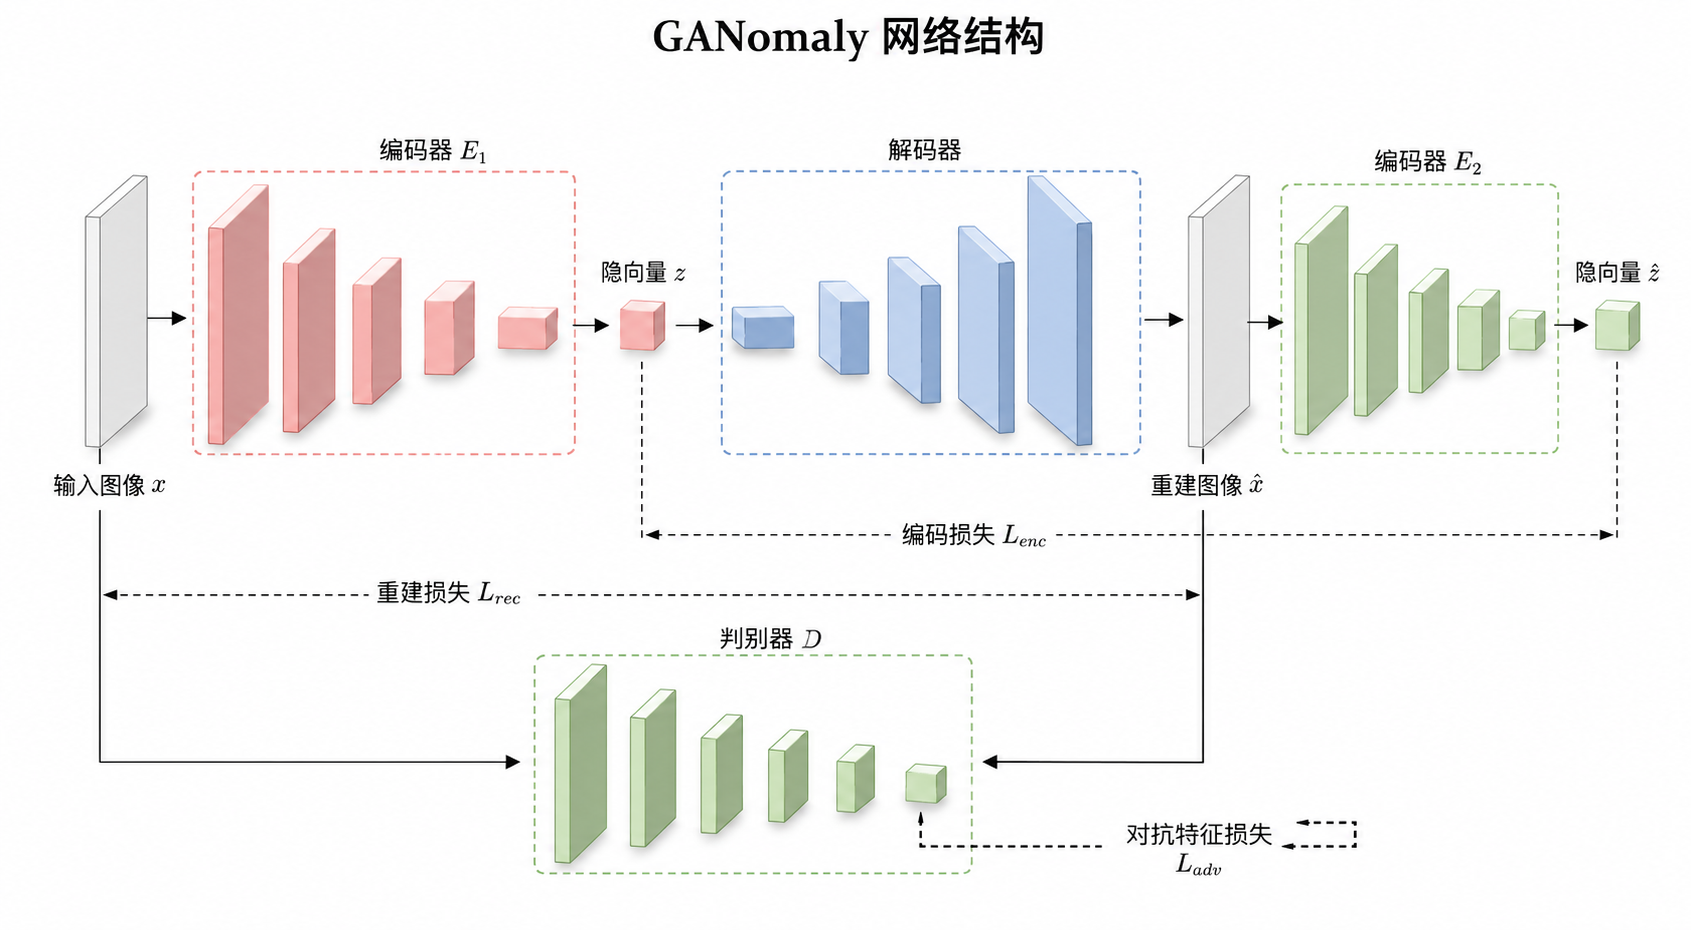
\includegraphics[width=0.95\linewidth]{images/ganomaly-3d-cn.png}
\caption{GANomaly 网络结构示意图}
\label{fig:ganomaly}
\end{figure}

\begin{table}[H]
\centering
\caption{GANomaly 模型说明}
\begin{tabularx}{\linewidth}{L{3.2cm}Y}
\toprule
\textbf{问题} & \textbf{说明} \\
\midrule
输入与输出 & 输入为 $[B,3,64,64]$；生成器输出同尺寸重建图，两个编码器分别输出 $[B,128,1,1]$ 的 $z$ 与 $\hat z$ \\
关键模块 & 编码器一把原图压缩为 $z$，解码器由 $z$ 重建 $\hat x$，参数独立但结构相同的编码器二把 $\hat x$ 编为 $\hat z$；判别器同时输出真假概率与中间特征 \\
训练信号 & 生成器使用 L1 重建损失、潜变量 MSE 和判别器特征 MSE，权重为 $40:1:1$；判别器使用真实图为 1、重建图为 0 的 BCE \\
异常分数 & 每块采用 $z$ 与 $\hat z$ 的平均绝对差；整图同时报告四块分数的最大值与平均值 \\
自己的理解 & 模型只用正常图训练，因而正常纹理应能稳定经历“编码--重建--再编码”；异常纹理若偏离正常分布，通常会使两个潜变量不一致，从而得到更高分数 \\
\bottomrule
\end{tabularx}
\end{table}

\subsubsection{训练目标与异常评分}

本项目 GANomaly 基线的三个生成器损失分别为
\begin{align}
\mathcal{L}_{\mathrm{rec}}&=\operatorname{mean}\left(|x-\hat{x}|\right),\\
\mathcal{L}_{\mathrm{enc}}&=\operatorname{mean}\left((z-\hat{z})^2\right),\\
\mathcal{L}_{\mathrm{adv}}&=\operatorname{mean}\left(
\left[\phi_D(\hat{x})-\operatorname{stopgrad}(\phi_D(x))\right]^2\right).
\end{align}
其中，重建项使用 L1 均值，编码项和判别器特征项使用 MSE。生成器总损失为
\begin{equation}
\mathcal{L}_{G}=40\mathcal{L}_{\mathrm{rec}}
+\mathcal{L}_{\mathrm{enc}}+\mathcal{L}_{\mathrm{adv}}.
\end{equation}
判别器使用二元交叉熵：
\begin{equation}
\mathcal{L}_{D}=\frac{1}{2}\left[
\operatorname{BCE}(D(x),1)+\operatorname{BCE}(D(\hat{x}),0)
\right].
\end{equation}
测试时每个裁剪块的异常分数为
\begin{equation}
A_{\mathrm{GAN}}(x)=\operatorname{mean}|z-\hat{z}|.
\end{equation}
一张原图的四个裁剪块分别得到 $A_1,\ldots,A_4$，本项目固定同时报告
\begin{equation}
A_{\max}=\max_i A_i,
\qquad
A_{\mathrm{mean}}=\frac{1}{4}\sum_{i=1}^{4}A_i.
\end{equation}
两种聚合产生两套整图排序，因此各自计算出的 AUROC 可能不同。

\subsection{MF-GANomaly}

\subsubsection{基本原理}

MF-GANomaly 是在 GANomaly 基础上提出的多特征异常检测方法。原版 GANomaly 最终主要利用高度压缩的潜变量 $z$ 与 $\hat z$ 判断异常，这种深层表示善于概括整体结构，却可能在压缩过程中弱化断丝、弯曲和局部纹理错位等细小异常。MF-GANomaly 因此保留原有的“编码--重建--再次编码”主流程，同时增加原图与重建图在像素层面和浅层特征层面的比较，使模型兼顾整体语义与局部纹理。

具体而言，第一编码器从输入图 $x$ 得到潜变量 $z$ 和第一层浅层特征 $f_1(x)$，解码器根据 $z$ 生成重建图 $\hat{x}$，第二编码器再从 $\hat{x}$ 得到 $\hat z$ 和 $f_1(\hat{x})$。两个编码器结构相同但参数相互独立。像素差异反映图像表面的重建偏差，浅层特征差异重点反映边缘、线条和周期纹理变化，深层编码差异则描述整体表示是否一致；三类信息互相补充。本项目采用论文式编码器变体：基线已有的中间卷积层继续使用 Batch Normalization（BN）和 LeakyReLU，并在第一层与最后一层卷积后也加入 BN 和 LeakyReLU，使各层特征的数值分布在训练中更稳定。

判别器的作用与 GANomaly 基线相同。它使用真实正常图作为真样本、生成器重建图作为假样本，通过二元交叉熵学习区分二者；其分类头之前的内部特征还用于生成器的特征匹配损失，促使重建图在判别器看来更接近真实正常图。训练时，生成器综合优化像素距离、浅层特征距离、潜变量距离和判别器特征距离，判别器与生成器仍按 batch 交替更新。

需要区分训练损失和测试异常分数：训练损失用于反向传播并修改网络参数，而测试分数只在模型训练完成后衡量样本偏离正常模式的程度，不参与梯度计算。本项目的测试分数直接合并像素、浅层特征和深层编码三种差异；分数越大，表示输入越难被模型按照正常纹理规律稳定重建与编码，因此越可能是异常图像。

\begin{figure}[H]
\centering
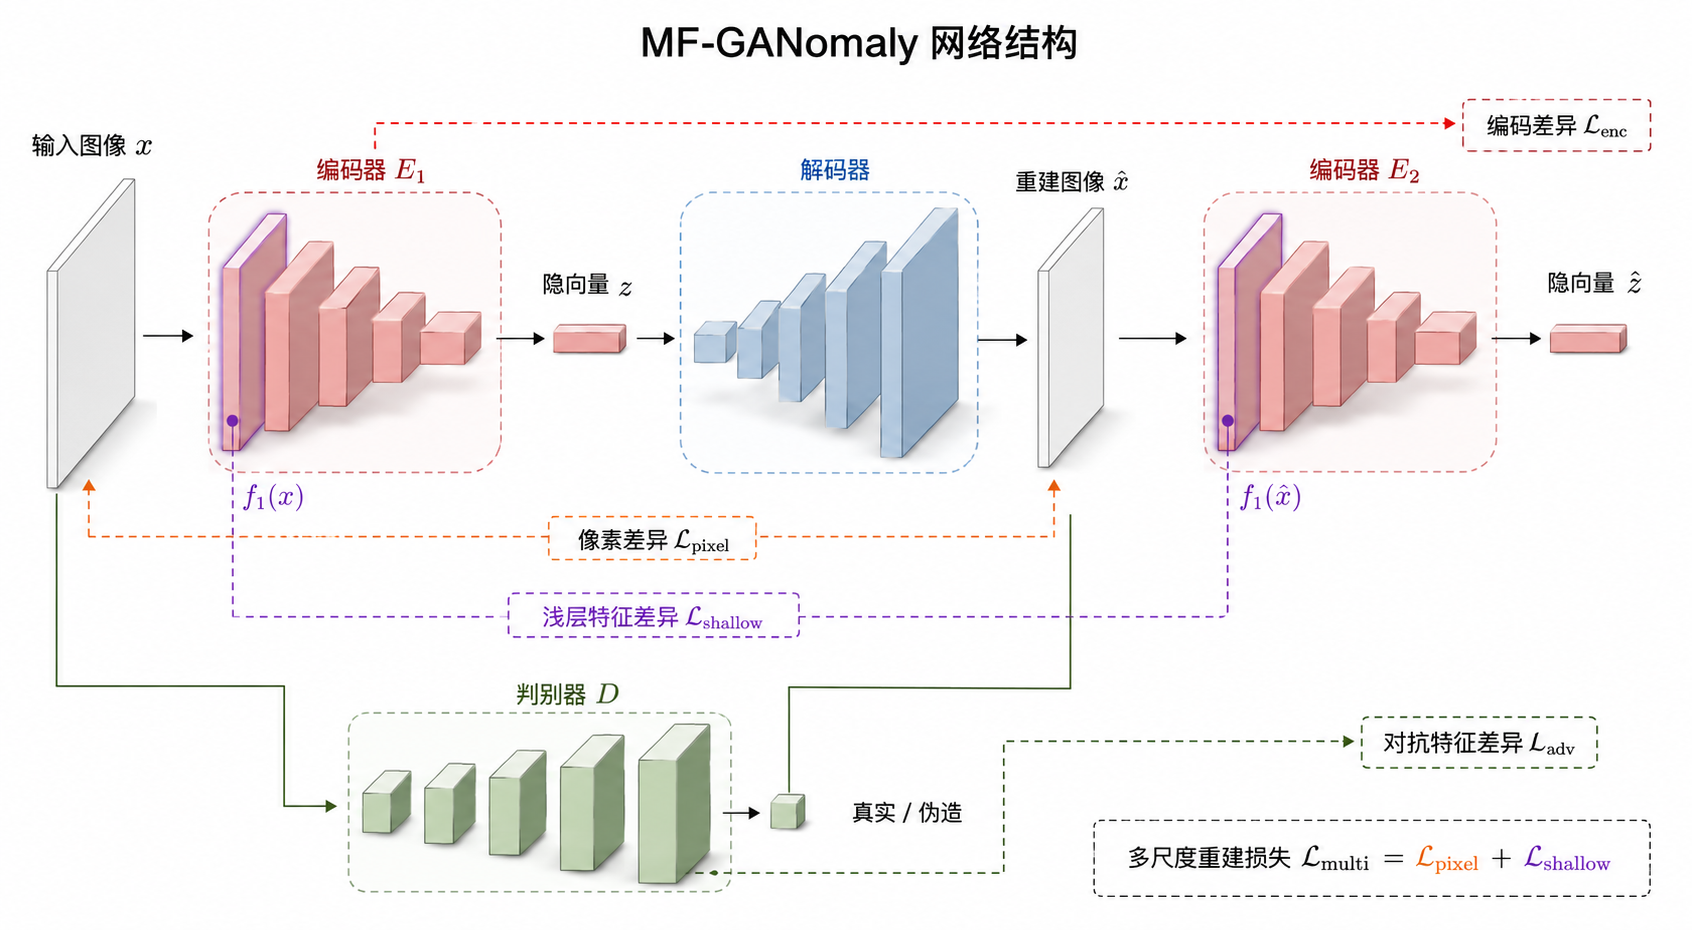
\includegraphics[width=0.95\linewidth]{images/mf-ganomaly-3d-cn.png}
\caption{MF-GANomaly 网络结构示意图}
\label{fig:mfganomaly}
\end{figure}

\begin{table}[H]
\centering
\caption{MF-GANomaly 相对基线的改动}
\begin{tabularx}{\linewidth}{L{3.2cm}Y}
\toprule
\textbf{问题} & \textbf{说明} \\
\midrule
改动位置 & 两个编码器除返回最终潜变量外，还返回第一层卷积后的 $[B,64,32,32]$ 浅层特征 \\
新增损失 & 将原图与重建图的像素 L2 距离、两侧第一层浅层特征 L2 距离相加，构成多特征重建项 \\
归一化与激活 & 编码器各卷积层后采用 BN 与 LeakyReLU；相较基线，本项目的论文式变体还为第一层和最后一层补充这两个操作 \\
预期作用 & 深层潜变量偏向整体语义，第一层仍保留边缘、周期纹理和局部细节，因此对断丝、弯曲等小缺陷更敏感 \\
实现差异 & 论文对“多尺度”的具体取层和跨块聚合未完全公开；本项目明确使用第一层浅特征，按逐样本 L2 范数实现，并同时报告最大值与平均值聚合 \\
\bottomrule
\end{tabularx}
\end{table}

\subsubsection{关键公式}

MF-GANomaly 在像素重建距离之外加入两个编码器第一层浅特征的距离：
\begin{equation}
\mathcal{L}_{\mathrm{shallow}}
=\left\lVert f_1(x)-f_1(\hat{x})\right\rVert_2,
\qquad
\mathcal{L}_{\mathrm{con}}
=\lVert x-\hat{x}\rVert_2+\mathcal{L}_{\mathrm{shallow}}.
\end{equation}
训练时仍采用重建项、编码项和判别器特征项的 $40:1:1$ 加权组合；本项目测试分数为
\begin{equation}
A_{\mathrm{MF}}(x)=\lVert z-\hat z\rVert_2
+40\left(\lVert x-\hat x\rVert_2
+\lVert f_1(x)-f_1(\hat x)\rVert_2\right).
\end{equation}

编码器中的 BN 对每个特征通道分别计算一个 mini-batch 内（同时包含该通道各空间位置）的均值与方差。设该通道参与统计的元素数为 $m$，输入为 $u_1,\ldots,u_m$，则
\begin{align}
\mu_B&=\frac{1}{m}\sum_{i=1}^{m}u_i,
&
\sigma_B^2&=\frac{1}{m}\sum_{i=1}^{m}(u_i-\mu_B)^2,\\
\hat{u}_i&=\frac{u_i-\mu_B}{\sqrt{\sigma_B^2+\epsilon}},
&
y_i&=\gamma\hat{u}_i+\beta.
\end{align}
其中，$\epsilon$ 防止分母为零，$\gamma$ 与 $\beta$ 是网络通过训练学习的缩放和偏移参数。BN 先把特征调整到较稳定的尺度，再允许网络利用 $\gamma$ 和 $\beta$ 学回合适的分布；它本身不是异常分数，也不会单独判断异常，而是帮助梯度传播和训练稳定。BN 后使用 LeakyReLU：
\begin{equation}
\operatorname{LeakyReLU}(a)=
\begin{cases}
a, & a\ge 0,\\
0.2a, & a<0,
\end{cases}
\end{equation}
从而在提供非线性的同时保留少量负半轴信息，降低神经元长期没有梯度的风险。

\subsection{\texorpdfstring{\hspace{0.5em}}{}Mask Encoders}

\subsubsection{基本原理}

GANomaly 类方法在训练时把完整正常图同时作为输入和重建目标，模型可能逐渐学会近似复制输入。若测试时也能把异常区域一并重建，原图与重建图之间的差异就会减小，从而造成漏检。Mask Encoders 通过人为遮挡正常图的一部分构造自监督任务：输入是中心区域缺失的正常图，监督目标则是遮挡前的完整正常图。由于缺失位置没有可供直接复制的像素，模型必须利用周围纹理和结构推断中心内容，从而学习正常 Grid 的排列规律，而无需人工标注异常位置。

模型采用单编码器--解码器生成器。编码器把 $[B,3,128,128]$ 的输入压缩为 $[B,512,1,1]$ 的潜变量，解码器再将其恢复为同尺寸重建图 $\hat{x}$。与 GANomaly 和 MF-GANomaly 不同，该模型没有第二编码器，不计算 $z$ 与 $\hat z$ 的编码损失，而是把学习重点放在遮挡补全和图像重建质量上。

训练分为两个阶段。第一阶段固定抽取 50\% 的正常裁剪块，将中心 $64\times64$ 区域遮挡，并以完整图为目标训练 80 轮；第二阶段继承第一阶段生成器和判别器权重，重新创建 Adam 优化器，再用全部完整正常裁剪块微调 80 轮。前一阶段学习根据上下文补全正常纹理，后一阶段把这种能力适配到测试时使用的完整图重建任务。

判别器把输入图逐层压缩为 100 维特征，再通过线性层和 Sigmoid 输出真假概率。它以完整正常图为真样本、生成器重建图为假样本进行训练；生成器则直接要求 $D(\hat{x})$ 接近 1。因此，判别器为生成器提供“重建图是否像真实正常图”的学习信号，补充单纯 L2 像素距离可能产生的模糊结果。两个网络在每个 batch 内交替更新。测试阶段不再更新参数，也不使用判别器概率作为异常分数，而是用原图与重建图的 L2 距离衡量异常程度。

\begin{figure}[H]
\centering
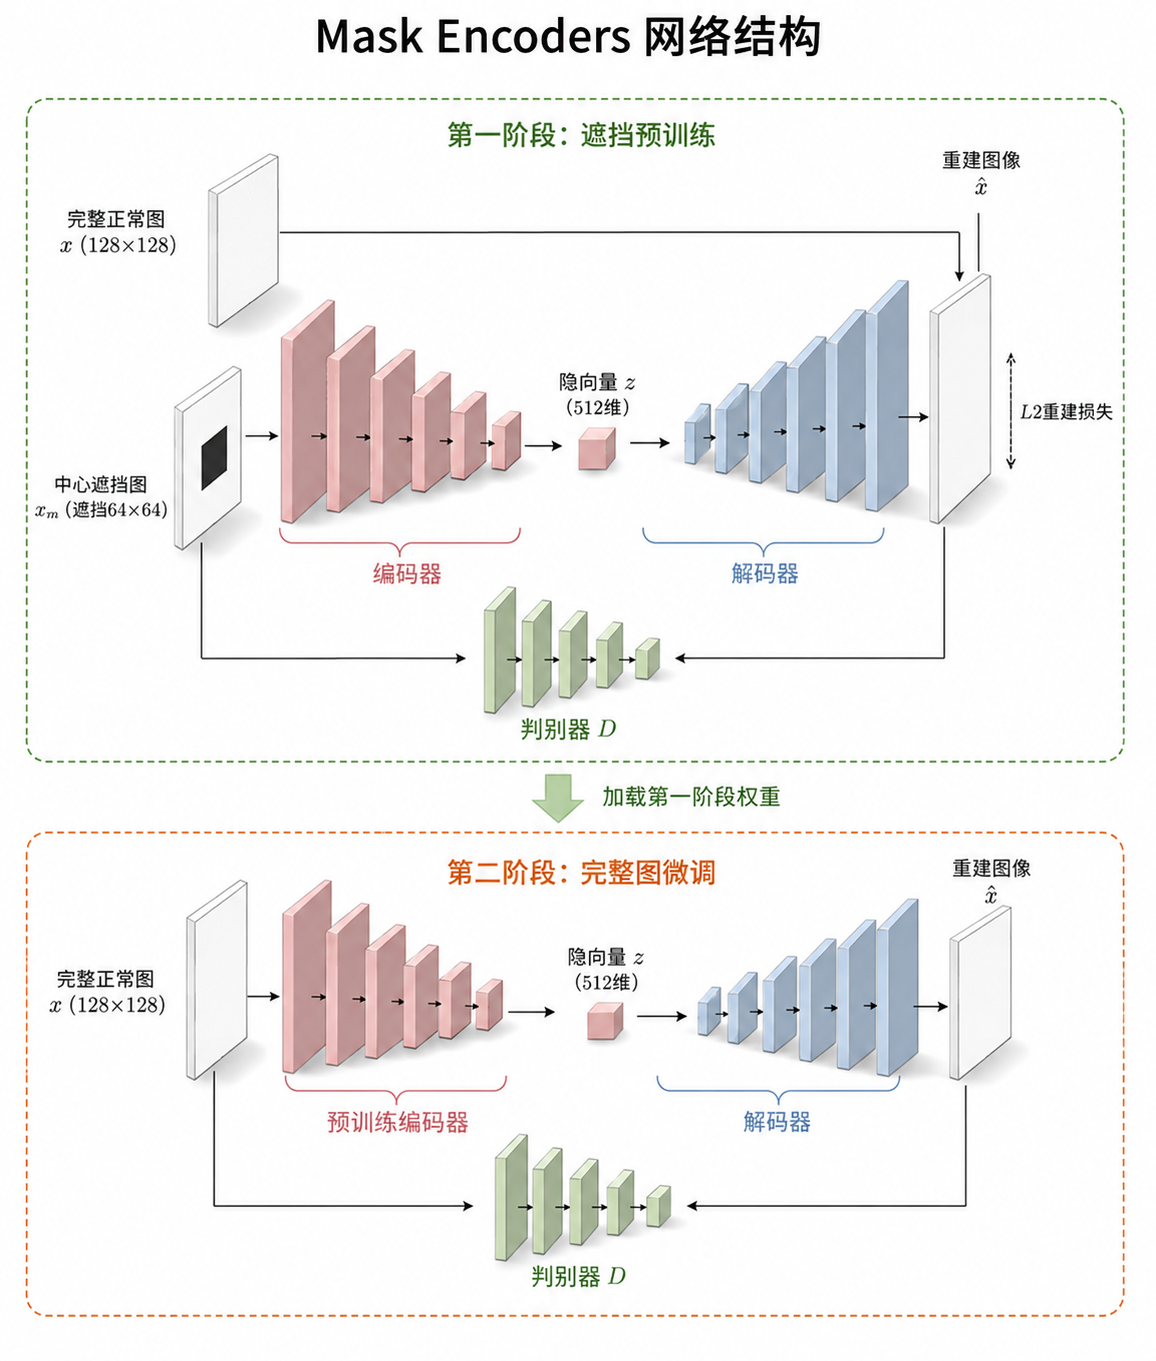
\includegraphics[width=0.95\linewidth]{images/mask-encoders-3d-cn.png}
\caption{Mask Encoders 两阶段训练结构示意图}
\label{fig:mask}
\end{figure}

\begin{table}[H]
\centering
\caption{Mask Encoders 两阶段训练}
\begin{tabularx}{\linewidth}{L{3.2cm}Y}
\toprule
\textbf{阶段} & \textbf{说明} \\
\midrule
第一阶段 & 固定抽取 50\% 的正常裁剪块，在 $128\times128$ 输入中心遮挡 $64\times64$ 区域，以未遮挡完整图为目标训练 80 轮 \\
第二阶段 & 载入第一阶段生成器与判别器权重，重新创建 Adam 优化器，用全部完整正常裁剪块微调 80 轮 \\
预期作用 & 模型无法从遮挡区域直接复制像素，只能利用周围正常纹理推断缺失内容，因此被迫学习 Grid 的结构规律；第二阶段再适配完整图重建任务 \\
测试评分 & 每块异常分数为原图与重建图的 L2 距离；额外统计裁剪块 PSNR 与 SSIM，整图 AUROC 同时使用四块最大值和平均值 \\
\bottomrule
\end{tabularx}
\end{table}

\subsubsection{关键公式}

第一阶段的遮挡输入可概括为
\begin{equation}
x_{\mathrm{mask}}=x\odot M.
\end{equation}
概念上 $M=0$ 表示遮挡位置、$M=1$ 表示保留位置；实际代码因输入已归一化到 $[-1,1]$，直接把中心 $64\times64$ 区域填为 $-1$。无论输入是第一阶段的遮挡图还是第二阶段的完整图，监督目标 $x$ 均为完整正常图。每个样本的 L2 重建距离为
\begin{equation}
d_2(x,\hat{x})=\lVert x-\hat{x}\rVert_2
=\sqrt{\sum_j(x_j-\hat{x}_j)^2},
\end{equation}
其中 $j$ 遍历一张裁剪图的全部通道和空间位置。生成器的重建项、对抗项与总损失分别为
\begin{align}
\mathcal{L}_{\mathrm{rec}}&=\operatorname{mean}_{x\in B}d_2(x,\hat{x}),\\
\mathcal{L}_{\mathrm{adv}}&=\operatorname{BCE}(D(\hat{x}),1),\\
\mathcal{L}_{G}^{\mathrm{Mask}}&=40\mathcal{L}_{\mathrm{rec}}+\mathcal{L}_{\mathrm{adv}}.
\end{align}
其中，对抗项的目标标签为 1，表示生成器希望判别器把重建图判断为真实图。判别器损失为
\begin{equation}
\mathcal{L}_{D}^{\mathrm{Mask}}
=\frac{1}{2}\left[
\operatorname{BCE}(D(x),1)
+\operatorname{BCE}(D(\operatorname{stopgrad}(\hat{x})),0)
\right].
\end{equation}
更新判别器时对 $\hat{x}$ 使用 $\operatorname{stopgrad}$，使该步骤只修改判别器参数。测试时每个裁剪块的异常分数为
\begin{equation}
A_{\mathrm{Mask}}(x)=d_2(x,\hat{x})=\lVert x-\hat{x}\rVert_2.
\end{equation}
异常图若不能被模型按照正常纹理规律稳定重建，通常会得到更大的距离和异常分数。

\subsection{TS-GAN}

\subsubsection{基本原理}

前三种方法只利用正常图片训练，能够学习正常模式，却没有使用现实中可能已经收集到的少量异常样本。TS-GAN 采用弱监督双流结构，同时建立正常生成器 $G_N$ 和异常生成器 $G_A$：前者学习正常图的重建规律，后者利用少量已知异常图学习异常模式。两个生成器结构相同但参数完全独立，避免第二阶段的异常训练直接改变正常生成器，使正常支路仍能作为稳定参照。

两条生成器都由编码器和解码器构成，并加入一条跳跃连接。编码器把 $[B,3,64,64]$ 的输入压缩成 $[B,512,1,1]$ 的潜变量；编码器第 4 层的 $[B,512,4,4]$ 特征与解码器第一层的同尺寸输出沿通道维拼接，得到 $[B,1024,4,4]$，再继续解码。潜变量提供高度压缩的整体信息，跳跃特征则向解码端补充局部空间结构和纹理细节。

训练分为两个阶段。第一阶段用正常裁剪块训练 $G_N$ 与共享判别器 $D$ 共 150 轮；此时 $G_A$ 保持冻结。第二阶段冻结已经训练好的 $G_N$，从 Grid 五类缺陷中各取 2 张、合计 10 张异常原图训练 $G_A$ 与同一个 $D$ 共 50 轮。共享判别器继承第一阶段模型参数，但第二阶段重新建立 Adam 优化器。判别器始终判断“真实输入还是生成器重建图”，并不直接分类正常与异常：第二阶段的真实异常图标签仍为 1，因为这里的 1 表示真实图片。

测试时，同一输入分别经过 $G_N$ 和 $G_A$，得到正常支路差异 $S_N$ 与异常支路差异 $S_A$。正常图通常容易被 $G_N$ 重建而得到较小的 $S_N$；异常图通常更难被 $G_N$ 重建，同时更接近 $G_A$ 学过的异常模式，因此 $S_N$ 较大而 $S_A$ 较小。最终使用 $S_N-0.1S_A$ 排序，使异常支路成为正常支路的对照参照。

\begin{figure}[H]
\centering
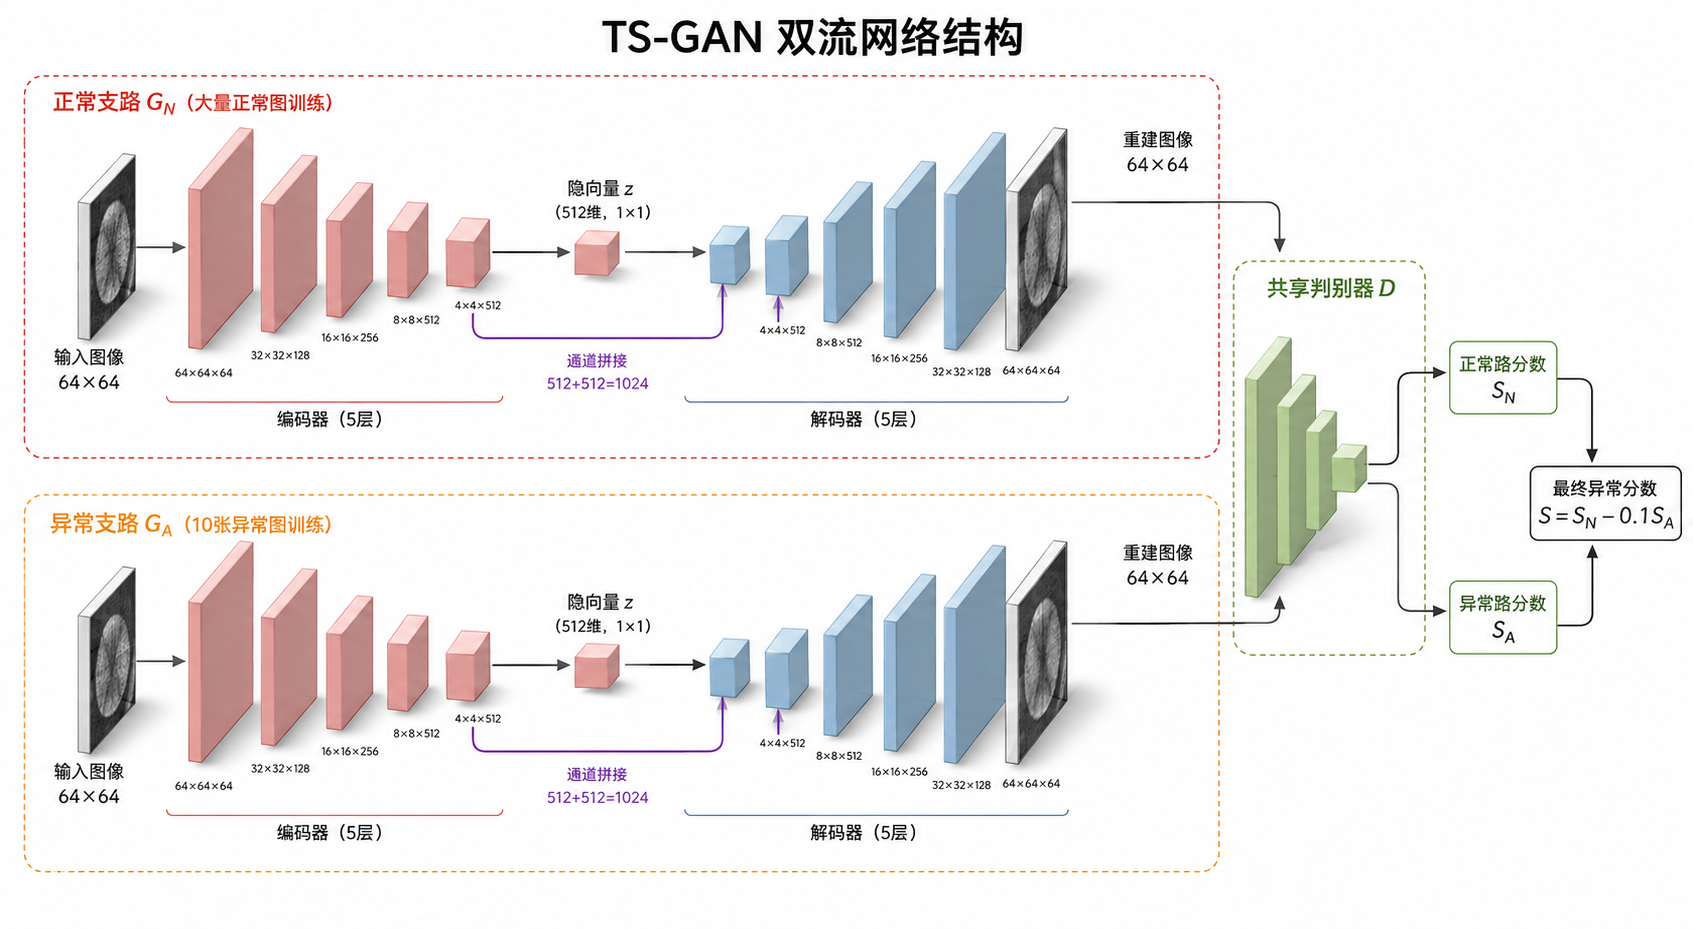
\includegraphics[width=0.95\linewidth]{images/ts-gan-3d-cn.png}
\caption{TS-GAN 双流结构示意图}
\label{fig:tsgan}
\end{figure}

\begin{table}[H]
\centering
\caption{TS-GAN 双流模型说明}
\begin{tabularx}{\linewidth}{L{3.2cm}Y}
\toprule
\textbf{问题} & \textbf{说明} \\
\midrule
正常支路 & 第一阶段只用正常裁剪块训练正常生成器与共享判别器 150 轮，生成器损失含重建、判别器特征和对抗项 \\
异常支路 & 第二阶段冻结正常生成器；按种子 42 从五类缺陷各选 2 张异常图，共 10 张，训练异常生成器与同一判别器 50 轮 \\
共享部分 & 两个生成器参数互不共享；同一判别器在不同阶段分别接收真实输入和对应支路重建图，其特征既参与生成器损失也参与测试评分 \\
跳跃连接 & 编码器第 4 层 $[B,512,4,4]$ 与解码器第 1 层输出 $[B,512,4,4]$ 沿通道维拼接为 $[B,1024,4,4]$，向解码端补充空间细节 \\
训练权重 & 正常与异常生成器训练时均采用重建、判别器特征、直接对抗三项损失，权重为 $40:1:1$；两阶段学习率分别为 0.0002 和 0.0001 \\
最终分数 & 正常支路分数 $S_N$ 减去 $0.1$ 倍异常支路分数 $S_A$；若输入更像异常支路学过的异常模式，$S_A$ 较小，最终异常分数仍相对升高 \\
\bottomrule
\end{tabularx}
\end{table}

\subsubsection{关键公式}

设当前训练支路为 $b\in\{N,A\}$，其生成器输出为 $\hat{x}_b$。两条支路训练时使用相同形式和相同权重的生成器损失：
\begin{align}
\mathcal{L}_{\mathrm{rec}}^{(b)}
&=\operatorname{mean}_{x\in B}\lVert x-\hat{x}_b\rVert_2,\\
\mathcal{L}_{\mathrm{fea}}^{(b)}
&=\operatorname{mean}_{x\in B}
\lVert\operatorname{stopgrad}(\phi_D(x))-\phi_D(\hat{x}_b)\rVert_2,\\
\mathcal{L}_{\mathrm{adv}}^{(b)}
&=\operatorname{BCE}(D(\hat{x}_b),1),\\
\mathcal{L}_{G_b}
&=40\mathcal{L}_{\mathrm{rec}}^{(b)}
+\mathcal{L}_{\mathrm{fea}}^{(b)}
+\mathcal{L}_{\mathrm{adv}}^{(b)}.
\end{align}
这里必须区分训练权重和测试权重：异常生成器训练时的重建权重也是 40，而不是 10。判别器在当前支路上的损失为
\begin{equation}
\mathcal{L}_{D}^{(b)}
=\frac{1}{2}\left[
\operatorname{BCE}(D(x),1)
+\operatorname{BCE}(D(\operatorname{stopgrad}(\hat{x}_b)),0)
\right].
\end{equation}
测试阶段不再使用 BCE，而是分别计算正常支路和异常支路分数：
\begin{align}
S_N(x)&=40\lVert x-\hat{x}_N\rVert_2
+\lVert\phi_D(x)-\phi_D(\hat{x}_N)\rVert_2,\\
S_A(x)&=10\lVert x-\hat{x}_A\rVert_2
+\lVert\phi_D(x)-\phi_D(\hat{x}_A)\rVert_2.
\end{align}
最终异常分数为
\begin{equation}
S(x)=S_N(x)-\eta S_A(x),\qquad \eta=0.1.
\end{equation}
其中，测试参数 $\alpha=40$、$\beta=10$ 分别控制两条支路中像素距离相对判别器特征距离的权重，$\eta=0.1$ 控制异常支路对最终结果的影响。这三个数用于测试评分组合，不会反向传播修改模型参数。

\subsubsection{论文式像素定位方法}

图片级异常分数用于判断整张图片是否异常，像素定位则采用论文单独描述的滑动窗口 PSNR 方法。对于 Grid 测试图，首先只使用正常生成器得到重建图 $\hat{x}_N=G_N(x)$。设原图与重建图共有 $n$ 个像素值，像素范围为 $[0,1]$，则均方误差和峰值信噪比分别为
\begin{align}
\operatorname{MSE}(x,\hat{x}_N)
&=\frac{1}{n}\sum_{i=1}^{n}(x_i-\hat{x}_{N,i})^2,\\
\operatorname{PSNR}(x,\hat{x}_N)
&=10\log_{10}\left(\frac{1}{\operatorname{MSE}(x,\hat{x}_N)}\right).
\end{align}
PSNR 越高，表示两张图越相似。先计算整个 $64\times64$ 裁剪块的整体 PSNR，记为 $P_{\mathrm{global}}$；再用窗口遍历裁剪块，在位置 $(i,j)$ 计算局部 PSNR $P_{\mathrm{local}}(i,j)$。异常响应定义为
\begin{equation}
H(i,j)=\max\left(P_{\mathrm{global}}-P_{\mathrm{local}}(i,j),0\right).
\end{equation}
若某个局部区域比整块图的平均水平重建得更差，其局部 PSNR 会降低，$H(i,j)$ 因而增大。所有响应最终按单张图片归一化到 $[0,1]$ 并绘制为连续热图。论文没有给出二值化阈值，也没有公开窗口大小、步长和重叠窗口的汇总方式；本项目采用窗口边长 8、步长 1，并将覆盖同一像素的窗口响应取平均。这些参数属于明确记录的复现假设，不作为论文原始设定。

\subsection{四个模型的关系}

\begin{table}[H]
\centering
\caption{四个模型对比}
\small
\begin{tabularx}{\linewidth}{L{2.4cm}C{1.5cm}C{1.7cm}C{1.6cm}Y}
\toprule
\textbf{模型} & \textbf{正常数据} & \textbf{异常数据} & \textbf{训练阶段} & \textbf{主要改进} \\
\midrule
GANomaly & 是 & 否 & 一阶段 & 双编码器重建基线 \\
MF-GANomaly & 是 & 否 & 一阶段 & 增加浅层多特征约束 \\
Mask Encoders & 是 & 否 & 两阶段 & 遮挡补全预训练与完整图微调 \\
TS-GAN & 是 & 少量 & 两阶段 & 正常和异常双流生成器与共享判别器 \\
\bottomrule
\end{tabularx}
\end{table}

\section{统一符号与评价指标}

\subsection{符号定义}

\begin{longtable}{L{2.7cm}L{3.5cm}L{6.5cm}}
\caption{关键符号说明}\\
\toprule
\textbf{符号} & \textbf{名称或形状} & \textbf{含义} \\
\midrule
\endfirsthead
\toprule
\textbf{符号} & \textbf{名称或形状} & \textbf{含义} \\
\midrule
\endhead
$x$ & $3\times64\times64$ 或 $3\times128\times128$ & 输入图像裁剪块 \\
$\hat{x}$ & 同 $x$ & 生成器重建的图像 \\
$z$ & GANomaly/MF 为 $128\times1\times1$；TS-GAN 为 $512\times1\times1$ & 第一编码器提取的潜变量 \\
$\hat{z}$ & 同 $z$ & 第二编码器对重建图的编码 \\
$D(\cdot)$ & 概率与特征 & 真假概率用于 BCE；分类头之前的特征用于特征匹配 \\
$f_l(\cdot)$ & 第 $l$ 层特征 & MF-GANomaly 使用的浅层特征 \\
$M$ & 掩码 & Mask Encoders 使用的二值遮挡图 \\
$S_N,S_A$ & 标量 & TS-GAN 正常支路与异常支路分数 \\
$A_{\max},A_{\mathrm{mean}}$ & 标量 & 四个裁剪块分数的最大值与平均值 \\
\bottomrule
\end{longtable}

\subsection{评价指标}

\begin{equation}
\mathrm{TPR}=\frac{\mathrm{TP}}{\mathrm{TP}+\mathrm{FN}},
\qquad
\mathrm{FPR}=\frac{\mathrm{FP}}{\mathrm{FP}+\mathrm{TN}}.
\end{equation}

ROC 曲线遍历全部可能阈值，横轴为 FPR，纵轴为 TPR；AUROC 是曲线下面积。直观上，它等于随机抽取一张异常图和一张正常图时，模型把异常图分数排得更高的概率。AUROC 不需要先固定分类阈值，0.5 约等于随机排序，越接近 1 越好。本报告现有主结果是图片级 AUROC；Mask Encoders 的 PSNR、SSIM 是裁剪块级计算后取均值。独立验证若报告 F1、精确率或召回率，必须先说明阈值来源。

\section{实现过程与训练设置}

\subsection{项目结构}

\begin{table}[H]
\centering
\caption{关键代码模块}
\begin{tabularx}{\linewidth}{L{4.2cm}Y L{2.2cm}}
\toprule
\textbf{文件或目录} & \textbf{职责} & \textbf{对应模型} \\
\midrule
\path{src/anomaly_reproduction/models.py} & 定义双编码器生成器和输出概率、特征图的判别器 & GANomaly \\
\path{src/anomaly_reproduction/models_mf.py} & 复用基线层定义，额外返回两个编码器的第一层浅特征 & MF-GANomaly \\
\path{src/anomaly_reproduction/models_mask.py} & 定义 $128\times128$ 的补全生成器和判别器 & Mask Encoders \\
\path{src/anomaly_reproduction/models_ts.py} & 定义两套独立生成器、单跳跃连接和共享判别器 & TS-GAN \\
\path{src/anomaly_reproduction/losses*.py} & 实现各模型生成器损失、判别器损失与异常评分组件 & 全部模型 \\
\path{src/anomaly_reproduction/evaluate*.py} & 生成裁剪块分数、整图聚合结果和 AUROC & 全部模型 \\
\bottomrule
\end{tabularx}
\end{table}

\subsection{统一超参数}

\begin{table}[H]
\centering
\caption{训练超参数}
\small
\begin{tabularx}{\linewidth}{L{2.3cm}C{2.2cm}C{1.8cm}C{1.8cm}C{2.7cm}}
\toprule
\textbf{参数} & \textbf{GANomaly} & \textbf{MF} & \textbf{Mask} & \textbf{TS-GAN} \\
\midrule
输入尺寸 & $64\times64$ & $64\times64$ & $128\times128$ & $64\times64$ \\
批大小 & 16 & 16 & 16 & 16 \\
训练轮数 & 150 & 150 & $80+80$ & $150+50$ \\
学习率 & 0.0002 & 0.0002 & 0.0002 & 0.0002/0.0001 \\
优化器 & Adam & Adam & Adam & Adam \\
随机种子 & 42 & 42 & 42 & 42 \\
\bottomrule
\end{tabularx}
\end{table}

\subsection{训练流程}

\begin{enumerate}
  \item 数据集只读取 Grid 正常训练图，固定四块裁剪、缩放并归一化；DataLoader 以 batch 16 打乱训练样本。
  \item 每个 batch 先用真实图和生成器重建图计算判别器 BCE，执行 \texttt{zero\_grad}、反向传播和判别器 Adam 更新；重建图在此步骤中与生成器计算图分离。
  \item 随后冻结判别器参数但保留其对输入的梯度，重新前向计算生成器损失，反向传播并更新生成器。两种网络因此在同一 batch 内交替学习。
  \item 每轮记录各损失，按固定间隔保存检查点，并在训练结束保存 \texttt{checkpoint\_final.pt}、历史文件和配置副本。
  \item 测试时每个裁剪块独立评分；按原始图片路径将四块重新分组，分别取最大值和平均值，再与图片级标签计算 AUROC。
\end{enumerate}

\subsection{与论文不一致或未公开的实现细节}

\begin{longtable}{C{1.1cm}L{3.7cm}L{4.4cm}L{4.0cm}}
\caption{复现假设与影响}\\
\toprule
\textbf{序号} & \textbf{论文描述} & \textbf{本项目选择} & \textbf{可能影响} \\
\midrule
\endfirsthead
\toprule
\textbf{序号} & \textbf{论文描述} & \textbf{本项目选择} & \textbf{可能影响} \\
\midrule
\endhead
1 & 四块分数聚合方式未明确 & 同时报告最大值与平均值 & 不同聚合可能改变图片级排序 \\
2 & TS-GAN 异常训练图名单未公开 & 每类随机抽取 2 张，种子 42 & 测试集组成与论文可能不同 \\
3 & MF-GANomaly 多尺度取层未完整公开 & 使用两个编码器第一层卷积特征，距离采用逐样本 L2 & 可能改变损失量级和对局部纹理的敏感度 \\
4 & Mask Encoders 判别器分类头细节未完全公开 & 将 100 维分类特征经线性层与 Sigmoid 变为单一概率 & 影响对抗训练强度，但保持真假二分类目标 \\
5 & 论文环境为 PyTorch 1.8/CUDA 11.4/RTX 2060 & 本项目使用 PyTorch 2.11/CUDA 12.8/RTX 5070 Laptop & 算子实现、随机性和训练速度可能不同 \\
\bottomrule
\end{longtable}

\section{实验设计与测试结果}

\subsection{评价问题与对照关系}

\begin{table}[H]
\centering
\caption{实验问题}
\begin{tabularx}{\linewidth}{C{1.1cm}Y Y}
\toprule
\textbf{序号} & \textbf{要回答的问题} & \textbf{对照或证据} \\
\midrule
1 & 四个模型是否复现出论文所述趋势 & 与论文报告值及基线比较 \\
2 & 模型是否能识别未参与训练的数据 & 独立验证集 AUROC 与分类案例 \\
3 & 模型在哪些缺陷上容易失败 & 按缺陷类别统计并分析误报、漏报 \\
4 & 四块最大值和平均值哪种更合适 & 在预先固定的验证协议下比较 \\
5 & TS-GAN 能否定位 Grid 缺陷区域 & 论文式滑窗 PSNR 热图、Pixel AUROC 与案例分析 \\
\bottomrule
\end{tabularx}
\end{table}

\subsection{Grid 首轮复现结果}

\begin{table}[H]
\centering
\caption{MVTec AD Grid 图片级结果}
\small
\begin{tabularx}{\linewidth}{L{2.7cm}C{1.8cm}C{2.2cm}C{2.2cm}C{2.0cm}}
\toprule
\textbf{模型} & \textbf{测试图片} & \textbf{最大值 AUROC} & \textbf{平均值 AUROC} & \textbf{论文值} \\
\midrule
GANomaly & 78 & 0.6817 & \textbf{0.7026} & 0.658 \\
MF-GANomaly & 78 & \textbf{0.7703} & 0.7510 & 0.740 \\
Mask Encoders & 78 & \textbf{0.9365} & 0.9056 & 0.785 \\
TS-GAN & 68 & \textbf{0.9534} & 0.9240 & 0.806 \\
\bottomrule
\end{tabularx}
\end{table}

\noindent\textbf{必要说明：}TS-GAN 使用 10 张异常图进行弱监督训练，并在测试时排除了这些图片，因此其测试集与其他三个模型不同。以上结果来自单个随机种子，不能直接作为严格的模型排名。

\begin{table}[H]
\centering
\caption{Mask Encoders 重建质量补充结果}
\begin{tabularx}{0.72\linewidth}{Y C{2.8cm} C{2.8cm}}
\toprule
\textbf{指标} & \textbf{本项目} & \textbf{论文值} \\
\midrule
裁剪块 PSNR 均值 & 24.2551 & 23.631 \\
裁剪块 SSIM 均值 & 0.7862 & 0.802 \\
\bottomrule
\end{tabularx}
\end{table}

从本轮结果看，MF-GANomaly 相比 GANomaly 的最大值 AUROC 提高 0.0886，说明浅层纹理约束在 Grid 上有效。Mask Encoders 与 TS-GAN 的数值明显高于本项目基线和论文表格值，但更高数值同时受到固定四块裁剪、实现细节和测试集组成影响，只能视为值得进一步验证的现象。GANomaly 在平均聚合下更高，其余三种方法在最大聚合下更高，说明聚合方法改变的是整图排序关系，而不是“平均值不应超过最大值”的数值常识：表中比较的是两套分数各自计算得到的 AUROC。

\subsection{TS-GAN 滑动窗口 PSNR 像素定位实验}

本实验读取 TS-GAN 第 50 轮异常阶段检查点，不重新训练模型；测试仍排除异常支路训练见过的 10 张异常图，共使用 21 张正常图和 47 张异常图。每个 $64\times64$ 裁剪块由正常支路重建，采用窗口边长 8、步长 1 计算滑动窗口 PSNR 响应，随后将四块热图拼接为 $128\times128$ 的展示结果。论文只展示连续异常热图，没有给出像素二值化阈值，因此本实验不生成预测掩码，也不报告依赖固定阈值的 Precision、Recall、F1 或 IoU。

\begin{table}[H]
\centering
\caption{TS-GAN 论文式 PSNR 热图的额外像素级评估}
\begin{tabularx}{0.78\linewidth}{Y C{2.8cm}}
\toprule
\textbf{评估范围} & \textbf{Pixel AUROC} \\
\midrule
全部 68 张测试图 & \textbf{0.9683} \\
弯曲（Bent） & 0.9855 \\
断裂（Broken） & 0.9888 \\
胶水附着（Glue） & 0.9343 \\
金属杂质（Metal contamination） & 0.9958 \\
毛线缠绕（Thread） & 0.9673 \\
\bottomrule
\end{tabularx}
\end{table}

\noindent\textbf{指标说明：}论文没有报告上述 Pixel AUROC，0.9683 是本项目在明确滑窗参数下增加的评价结果，不能写成论文复现值。它表示随机抽取一个真实异常像素和一个正常像素时，连续热图把异常像素排在更高位置的概率约为 96.83\%，并不表示 96.83\% 的像素都被正确分类。

\begin{figure}[H]
\centering
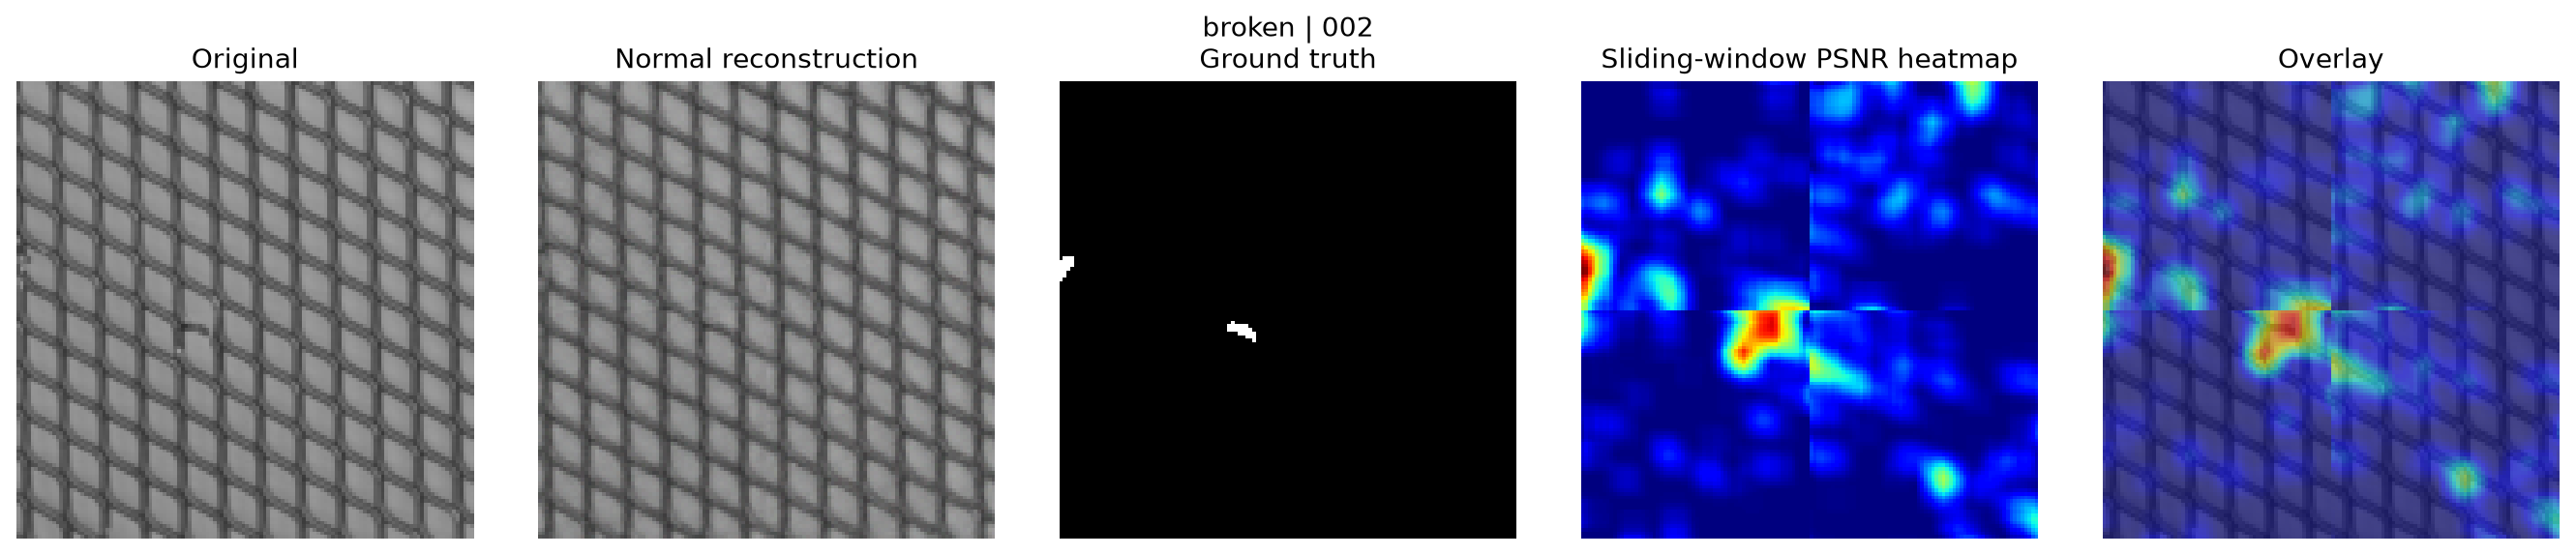
\includegraphics[width=\linewidth]{images/ts-gan-psnr-best-broken-002.png}
\caption{TS-GAN 在断裂样本上的滑窗 PSNR 热图示例。两个真实缺陷位置均出现集中高响应，但裁剪边界和少量正常纹理仍存在响应。}
\label{fig:tsgan-psnr-best}
\end{figure}

\begin{figure}[H]
\centering
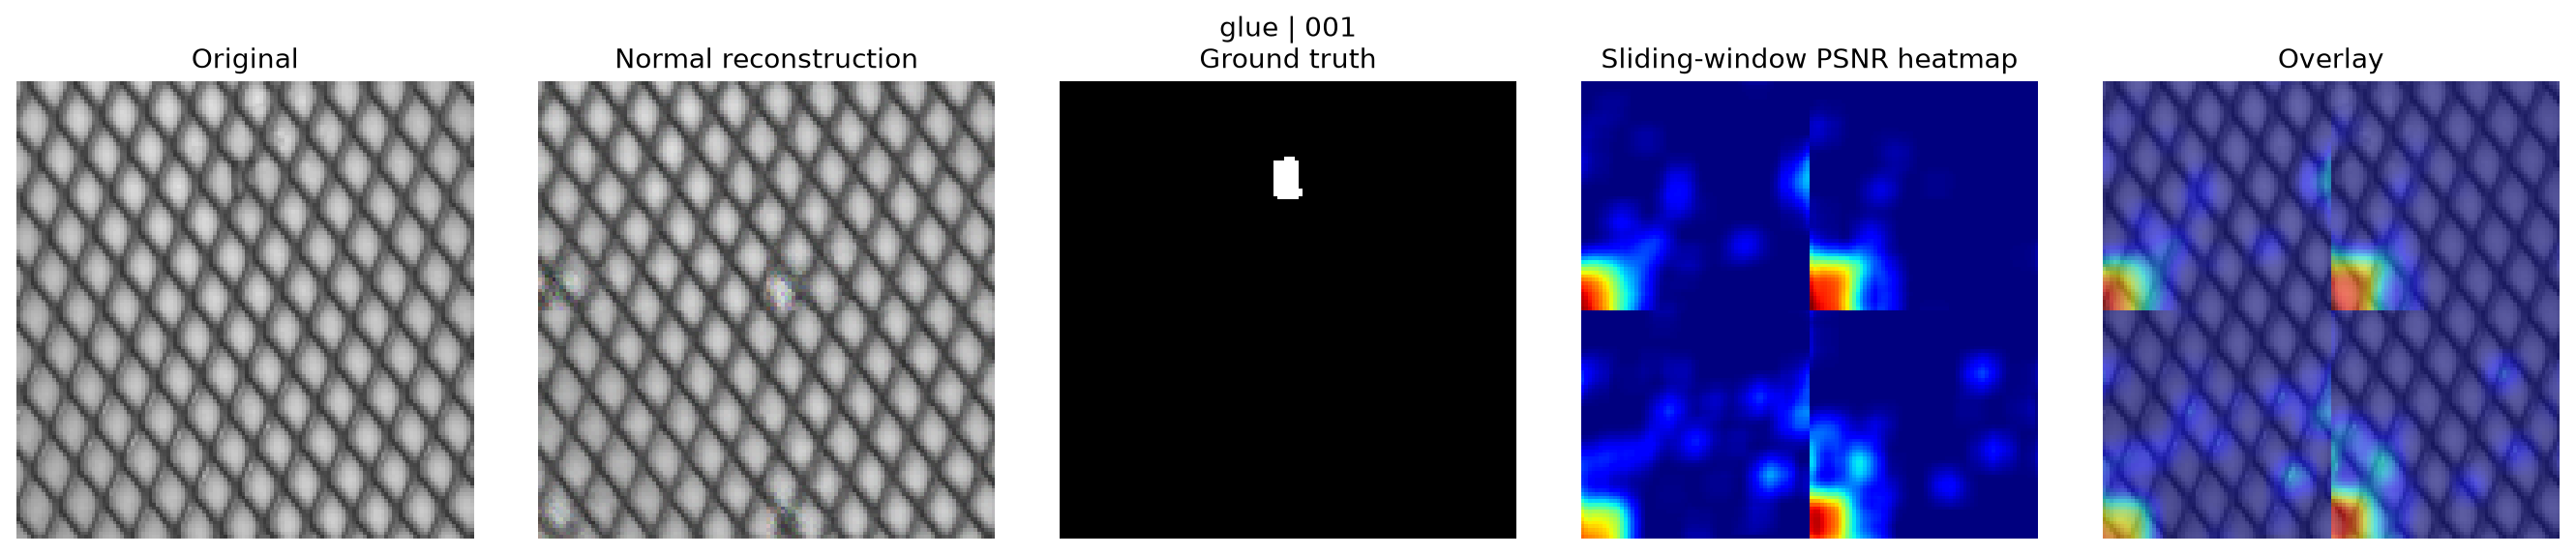
\includegraphics[width=\linewidth]{images/ts-gan-psnr-worst-glue-001.png}
\caption{TS-GAN 在胶水附着样本上的较差案例。该图单图 Pixel AUROC 为 0.6628，说明小尺寸、低对比度缺陷仍可能被纹理重建误差掩盖。}
\label{fig:tsgan-psnr-worst}
\end{figure}

总体结果明显好于此前采用逐像素双支路残差得到的噪声热图，说明论文采用局部窗口比较而非单像素比较是关键：窗口能够聚合邻域结构误差，而“整体 PSNR 减局部 PSNR”进一步突出相对整图平均水平重建明显较差的区域。不过，正常样本的纹理和四块拼接边界仍可能出现局部高响应；后续应在独立数据上验证，并进行窗口大小与步长的敏感性实验。

\subsection{未参与训练数据的定量结果}

\begin{table}[H]
\centering
\caption{TS-GAN 在 AITEX-AFID 上的零样本图片级结果}
\small
\begin{tabularx}{\linewidth}{L{2.2cm}C{1.7cm}C{1.6cm}C{1.6cm}C{1.6cm}C{1.6cm}Y}
\toprule
\textbf{汇总方式} & \textbf{AUROC} & \textbf{AP} & \textbf{准确率} & \textbf{F1} & \textbf{召回率} & \textbf{阈值} \\
\midrule
图块最大值 & 0.4463 & 0.4856 & 0.4953 & 0.0531 & 0.0283 & 2361.30 \\
图块平均值 & \textbf{0.5482} & \textbf{0.5392} & 0.5000 & 0.0536 & 0.0283 & 882.15 \\
\bottomrule
\end{tabularx}
\end{table}

\noindent 两种阈值均只由 35 张正常校准图的 0.99 分位数得到。最大值汇总的混淆矩阵为 TN=102、FP=4、FN=103、TP=3，平均值汇总为 TN=103、FP=3、FN=103、TP=3。虽然误报较少，但原因是阈值较高，代价是 106 张异常图中仅检出 3 张；因此约 0.50 的准确率不能解释为模型效果良好。与 Grid 上 0.9534（最大汇总）和 0.9240（平均汇总）的图片级 AUROC 相比，AITEX 分别下降 0.5071 和 0.3758，说明整图异常分数没有成功迁移到新的织物域。

\begin{table}[H]
\centering
\caption{AITEX-AFID 像素级总体结果}
\begin{tabularx}{0.88\linewidth}{Y C{2.8cm} C{2.8cm}}
\toprule
\textbf{评估范围} & \textbf{Pixel AUROC} & \textbf{Pixel AP} \\
\midrule
全部 211 张有像素评价资格的图像 & \textbf{0.7472} & 0.0060 \\
仅 105 张有掩码的异常图像 & 0.7475 & 0.0114 \\
\bottomrule
\end{tabularx}
\end{table}

\noindent Pixel AUROC 表示随机抽取一个异常像素和一个正常像素时，热图把异常像素排在更高位置的概率。AITEX 的 0.7472 比 Grid 的 0.9683 下降 0.2211，说明定位排序能力仍部分保留，但跨域后明显退化。Pixel AP 对稀少的异常像素更敏感；0.0060 表明热图虽然常在缺陷附近产生较高响应，却同时覆盖大量正常区域，精确定位能力较弱。Grid 实验未计算 Pixel AP，因此不能对该指标作直接数值比较。

\begin{table}[H]
\centering
\caption{AITEX-AFID 按缺陷类型的像素级结果}
\small
\begin{tabularx}{\linewidth}{C{1.2cm}L{3.2cm}C{1.2cm}C{2.2cm}C{2.2cm}}
\toprule
\textbf{代码} & \textbf{官方缺陷名称（中文释义）} & \textbf{图像数} & \textbf{Pixel AUROC} & \textbf{Pixel AP} \\
\midrule
002 & Broken end（断经） & 9 & 0.8170 & 0.005645 \\
006 & Broken yarn（断纱） & 8 & 0.8588 & 0.008655 \\
010 & Broken pick（断纬） & 10 & 0.6329 & 0.029709 \\
016 & Weft curling（纬纱卷曲） & 3 & 0.8887 & 0.007636 \\
019 & Fuzzyball（毛球） & 39 & 0.6773 & 0.000050 \\
022 & Cut selvage（切边缺陷） & 9 & 0.5851 & 0.000470 \\
023 & Crease（折痕） & 5 & 0.7563 & 0.002407 \\
025 & Warp ball（经纱结团） & 5 & 0.6641 & 0.000046 \\
027 & Knots（结头） & 1 & 0.8855 & 0.001299 \\
029 & Contamination（污染） & 1 & 0.7145 & 0.000497 \\
030 & Nep（棉结/纤维结粒） & 14 & 0.7753 & 0.000597 \\
036 & Weft crack（纬向裂缝） & 1 & 0.8235 & 0.468473 \\
\bottomrule
\end{tabularx}
\end{table}

\noindent 其中 002、030 等数字是 AITEX 文件名中的官方缺陷类型代码，不是模型分数。036 仅有 1 张图，其较高 AP 不具有稳定的类别统计意义；027、029 同样只有 1 张图，不能据此判断模型对这些缺陷具有稳定优势。

\subsection{表现较好的案例}

\begin{figure}[H]
\centering
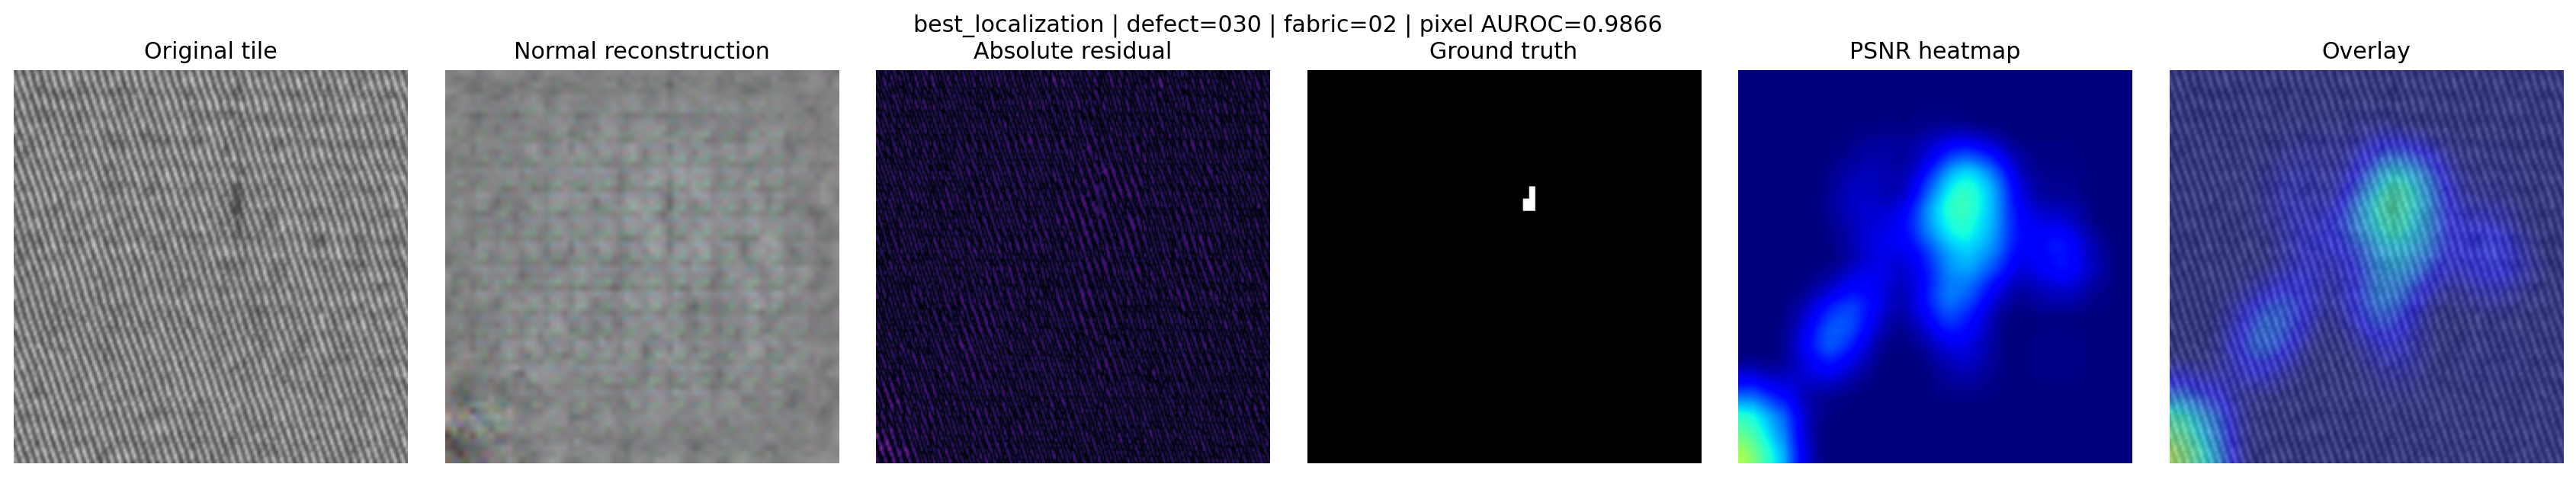
\includegraphics[width=\linewidth]{images/aitex-best-nep-0086.png}
\caption{AITEX 棉结缺陷 \texttt{0086\_030\_02} 的较好定位案例，单图 Pixel AUROC 为 0.9866。热图高响应覆盖真实缺陷附近，说明 Grid 上学习到的局部重建差异对部分跨域缺陷仍然有效；但 Pixel AP 仅为 0.0039，提示响应范围仍远大于真实掩码。}
\label{fig:aitex-best}
\end{figure}

\subsection{表现不理想的案例}

\subsubsection{误报案例}

\begin{figure}[H]
\centering
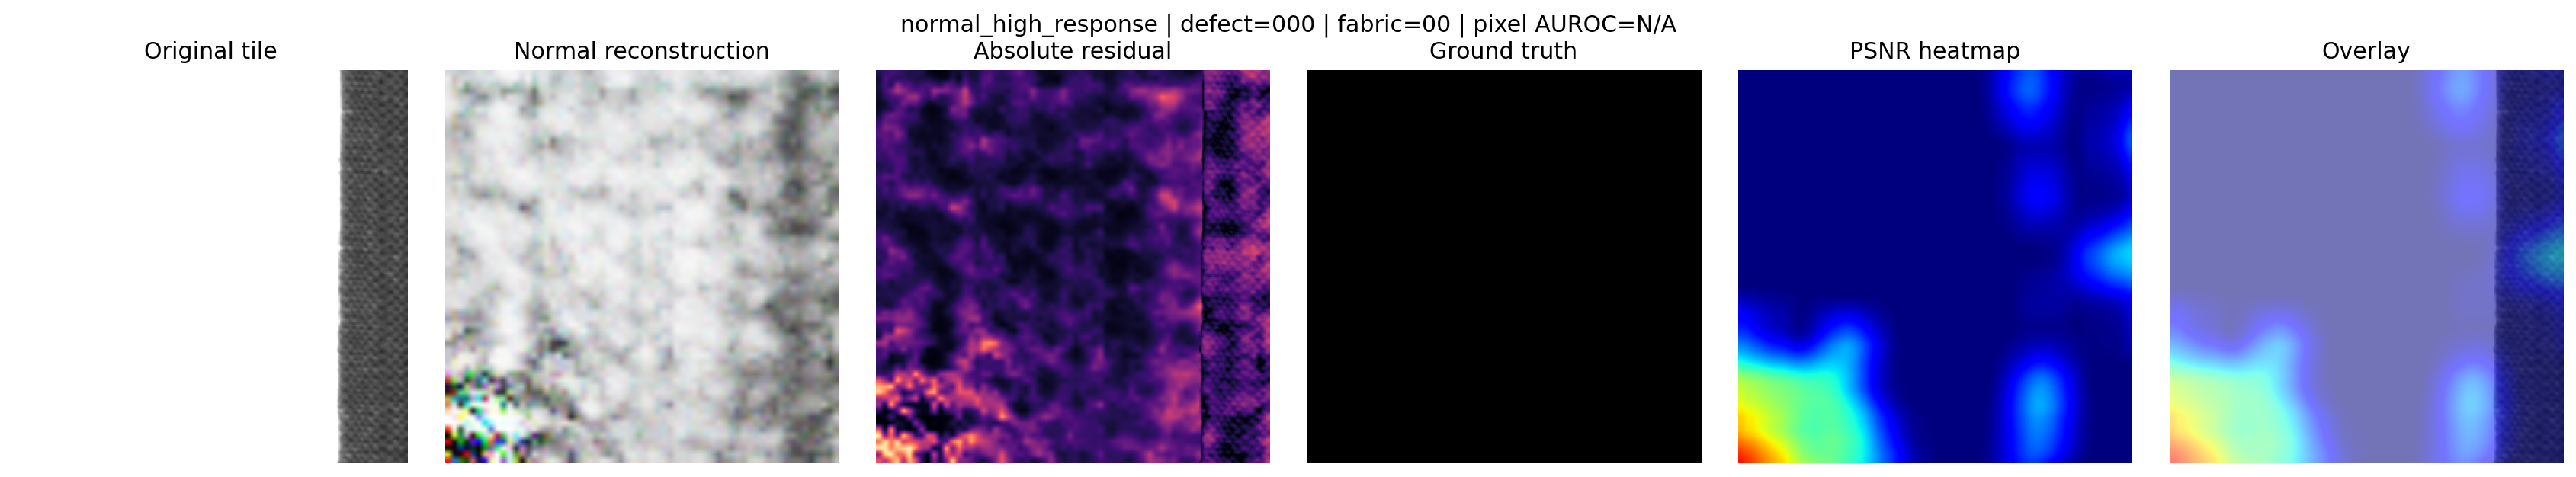
\includegraphics[width=\linewidth]{images/aitex-normal-high-response-0008.png}
\caption{AITEX 正常样本 \texttt{0008\_000\_00} 的高响应案例。真实掩码为空，但热图仍在正常纹理区域产生明显响应，说明材质变化和周期纹理的重建误差会被误当作缺陷证据。}
\label{fig:aitex-fp}
\end{figure}

\subsubsection{漏报案例}

\begin{figure}[H]
\centering
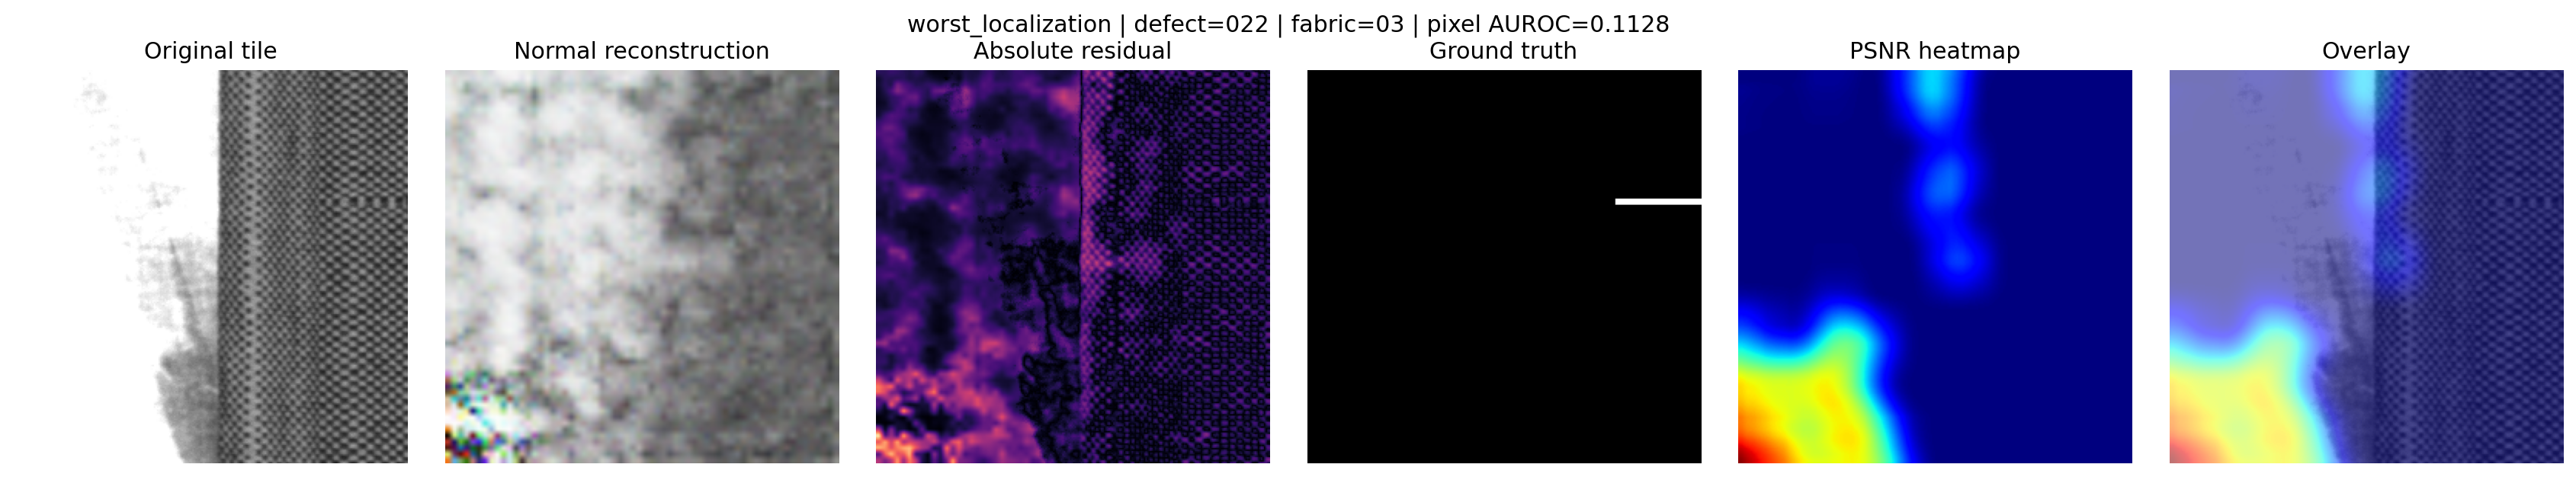
\includegraphics[width=\linewidth]{images/aitex-worst-cut-selvage-0104.png}
\caption{AITEX 切边缺陷 \texttt{0104\_022\_03} 的较差定位案例，单图 Pixel AUROC 仅为 0.1128。热图主要响应正常纹理而非真实缺陷，反映 $64\times64$ 输入分辨率、材质域偏移及单尺度窗口共同造成的定位失败。}
\label{fig:aitex-fn}
\end{figure}

\subsection{测试结果小结}

AITEX 独立验证不支持“Grid 上的高性能可以直接推广到其他织物数据”的结论。图片级平均汇总 AUROC 仅为 0.5482，且在正常校准阈值下只检出 3/106 张异常图，说明异常分数的尺度和排序均发生明显变化。像素级 Pixel AUROC 为 0.7472，表明局部 PSNR 热图仍保留部分位置排序能力；然而 Pixel AP 只有 0.0060，结合正常高响应与切边缺陷漏定位案例可知，热图存在大面积非缺陷响应。后续改进应优先考虑目标域正常样本适配、更高输入分辨率、多尺度窗口及基于正常目标域数据的热图校准，而不能使用 AITEX 异常测试标签反复选择参数。

\section{结果讨论}

\subsection{与论文结果的差异}

\begin{table}[H]
\centering
\caption{结果差异分析}
\begin{tabularx}{\linewidth}{L{3.2cm}Y Y}
\toprule
\textbf{差异来源} & \textbf{本项目情况} & \textbf{可能影响} \\
\midrule
框架与 CUDA 版本 & PyTorch 2.11.0+cu128；论文为 PyTorch 1.8.0、CUDA 11.4 & 算子实现、初始化与随机性可能改变训练轨迹 \\
数据预处理 & 固定四块裁剪后缩放 & 局部缺陷可能被放大，但跨块上下文会丢失 \\
随机种子 & 当前仅种子 42 & 无法估计均值和方差 \\
论文未公开细节 & 四块聚合、MF 具体取层、TS-GAN 异常图名单等由本项目明确设定 & 可能造成指标与论文不完全可比 \\
测试集组成 & TS-GAN 排除 10 张异常训练图 & 与其他模型不能直接严格比较 \\
\bottomrule
\end{tabularx}
\end{table}

\subsection{模型优势与不足}

\begin{itemize}
  \item \textbf{GANomaly：}结构和评分逻辑清晰，适合作为只用正常数据的基线；但仅以潜变量差异评分，可能忽略局部重建异常，对细小纹理缺陷较弱。
  \item \textbf{MF-GANomaly：}在基线中加入像素和浅层特征，使局部纹理变化更容易进入损失与评分；代价是损失量级、取层和权重更敏感，并增加特征计算。
  \item \textbf{Mask Encoders：}遮挡补全减少了直接复制输入的可能，本轮重建质量和 AUROC 均较好；但需要两阶段训练，中心遮挡任务与真实缺陷位置不完全一致，仍可能在边界或细小缺陷上失败。
  \item \textbf{TS-GAN：}少量异常样本使模型显式学习异常方向，本轮 Grid AUROC 最高；但结果依赖异常样本是否具有代表性，共享判别器在两阶段可能遗忘或饱和，且其测试集与无监督模型不同。AITEX 零样本结果进一步说明，这种优势并不会自动转化为跨数据域泛化能力。
\end{itemize}

\subsection{实验有效性威胁}

\begin{enumerate}
  \item \textbf{内部有效性：}当前同时报告最大与平均聚合，没有据测试结果删去较差方案；TS-GAN 的 10 张异常训练图已从测试中排除。但此前开发过程查看过测试 AUROC，因此后续独立数据才适合作为最终泛化证据。
  \item \textbf{外部有效性：}AITEX-AFID 验证扩展到了独立织物域，但目前只验证 TS-GAN，且未覆盖其他物体类别、相机和光照条件；因此仍不能将结论推广到一般工业异常检测。
  \item \textbf{统计有效性：}每个模型仅运行种子 42，缺少均值、标准差、置信区间及显著性检验，偶然初始化可能影响排序。
  \item \textbf{实现有效性：}论文未公开完整源码，本项目对多尺度取层、判别器分类头、异常训练图和图片聚合做了可复现假设，这些差异会影响与论文数值的严格比较。
\end{enumerate}

\section{结论与后续工作}

\subsection{主要结论}

\begin{enumerate}
  \item 四个模型已完成从数据读取、训练、检查点保存到图片级评估的完整流程；在 Grid、固定四块裁剪和种子 42 下，三个改进模型的 AUROC 均高于 GANomaly 基线。
  \item MF-GANomaly 的最佳 AUROC 为 0.7703，Mask Encoders 为 0.9365；与 GANomaly 的 0.7026 相比，结果支持浅层特征约束与遮挡补全在本实验协议下有效。
  \item TS-GAN 的最佳图片级 AUROC 为 0.9534，但它使用 10 张异常训练图且测试样本数为 68，不能与其余模型作完全公平的直接排名。按论文描述实现滑窗 PSNR 热图后，额外 Pixel AUROC 为 0.9683，说明该方法在当前 Grid 测试集上具有较好的像素排序能力；该数值不是论文报告值，且窗口参数仍属于复现假设。
  \item 在完全未重训练的 AITEX-AFID 外部验证中，TS-GAN 图片级最大、平均汇总 AUROC 分别为 0.4463 和 0.5482，Pixel AUROC 为 0.7472、Pixel AP 为 0.0060。与 Grid 结果的明显落差证明当前模型存在较强域依赖：局部定位排序能力部分保留，但整图异常识别和精确像素定位不能直接迁移。
\end{enumerate}

\subsection{后续工作}

\begin{itemize}
  \item 使用至少 3 个随机种子，报告均值和标准差。
  \item 固定统一测试集和预处理，对四个模型公平比较。
  \item 在 AITEX 正常训练子集上进行不使用异常标签的目标域适配，并与本报告的零样本结果严格区分。
  \item 对滑动窗口大小、步长和重叠响应汇总方式进行敏感性实验。
  \item 针对 AITEX 的正常高响应和细小缺陷漏定位，比较更高输入分辨率、多尺度窗口及正常域热图校准方法。
\end{itemize}

\clearpage
\section*{参考文献}
\addcontentsline{toc}{section}{参考文献}

\begin{enumerate}[label={[\arabic*]}]
  \item 步兆军. 基于自监督与弱监督学习的图像异常检测研究[D]. 南京：东南大学，2022.
  \item Akcay S, Atapour-Abarghouei A, Breckon T P. GANomaly: Semi-supervised anomaly detection via adversarial training[C]//Asian Conference on Computer Vision. Cham: Springer, 2018: 622--637.
  \item Bergmann P, Fauser M, Sattlegger D, et al. MVTec AD: A comprehensive real-world dataset for unsupervised anomaly detection[C]//Proceedings of the IEEE/CVF Conference on Computer Vision and Pattern Recognition. 2019: 9592--9600.
  \item Silvestre-Blanes J, Albero-Albero T, Miralles I, et al. AFID: A public fabric image database for defect detection[J]. AUTEX Research Journal, 2019. 数据集官网：\url{https://www.aitex.es/afid/}.
\end{enumerate}

\appendix
\clearpage
\section{关键代码整理与理解}

\noindent 本附录不建议粘贴完整工程。每段代码应只保留能说明关键算法的部分，并在代码前后解释输入、输出、张量形状和设计原因。

\subsection{代码片段记录表}

\begin{longtable}{L{3.7cm}L{2.5cm}L{3.0cm}L{4.0cm}}
\caption{关键代码索引}\\
\toprule
\textbf{文件与函数} & \textbf{输入输出} & \textbf{核心操作} & \textbf{自己的理解} \\
\midrule
\endfirsthead
\toprule
\textbf{文件与函数} & \textbf{输入输出} & \textbf{核心操作} & \textbf{自己的理解} \\
\midrule
\endhead
\fillin{例如 models.py Encoder.forward} & \fillin{形状} & \fillin{操作} & \fillin{为什么这样设计} \\
\fillin{训练一步函数} & \fillin{输入输出} & \fillin{反向传播与优化器} & \fillin{生成器和判别器如何交替} \\
\fillin{异常评分函数} & \fillin{输入输出} & \fillin{分数计算与聚合} & \fillin{评分与训练目标的关系} \\
\bottomrule
\end{longtable}

\clearpage
\subsection{关键代码一}

\noindent\textbf{文件与函数：}\fillin{路径和函数名}

\noindent\textbf{作用：}\fillin{一句话说明此代码解决什么问题}

\begin{lstlisting}[style=pythonstyle,caption={关键代码一},label={lst:key1}]
# Paste only the essential code here.
def key_function(inputs):
    outputs = ...
    return outputs
\end{lstlisting}

\noindent\textbf{逐步理解：}
\begin{enumerate}
  \item \fillin{输入张量的含义与形状。}
  \item \fillin{每个关键层或计算步骤做了什么。}
  \item \fillin{输出被哪个模块使用。}
  \item \fillin{如果删除或修改此代码，模型可能发生什么变化。}
\end{enumerate}

\subsection{关键代码二}

\noindent\textbf{文件与函数：}\fillin{路径和函数名}

\begin{lstlisting}[style=pythonstyle,caption={关键代码二},label={lst:key2}]
# Paste the discriminator or loss code here.
def compute_loss(...):
    loss = ...
    return loss
\end{lstlisting}

\noindent\textbf{自己的理解：}\fillin{不要逐字翻译代码，应解释数据如何流动、损失如何影响参数更新。}

\subsection{关键代码三}

\noindent\textbf{文件与函数：}\fillin{路径和函数名}

\begin{lstlisting}[style=pythonstyle,caption={关键代码三},label={lst:key3}]
# Paste the evaluation and score aggregation code here.
def anomaly_score(...):
    score = ...
    return score
\end{lstlisting}

\noindent\textbf{自己的理解：}\fillin{解释单个裁剪块得分怎样变成整张图片得分，以及 AUROC 如何使用这些分数。}

\section{完整配置与复现实验命令}

\subsection{配置文件}

\begin{lstlisting}[style=pythonstyle,caption={配置摘录}]
experiment:
  seed: 42
dataset:
  category: grid
  preprocessing: four_crops
  batch_size: 16
common_optimizer:
  name: Adam
  beta1: 0.5
  beta2: 0.999
ganomaly:
  image_size: 64
  latent_dim: 128
  epochs: 150
  learning_rate: 0.0002
mf_ganomaly:
  image_size: 64
  latent_dim: 128
  epochs: 150
  reconstruction_metric: l2
mask_encoders:
  image_size: 128
  mask_size: 64
  pretrain_fraction: 0.5
  epochs: [80, 80]
ts_gan:
  image_size: 64
  latent_dim: 512
  anomaly_images_per_type: 2
  epochs: [150, 50]
  learning_rates: [0.0002, 0.0001]
  evaluation: {alpha: 40, beta: 10, eta: 0.1}
\end{lstlisting}

\subsection{运行命令}

\begin{lstlisting}[style=pythonstyle,caption={训练和评估命令}]
python -m anomaly_reproduction.train_four_crops
python -m anomaly_reproduction.evaluate --config configs/ganomaly_grid_four_crops.yaml
python -m anomaly_reproduction.train_mf
python -m anomaly_reproduction.evaluate_mf
python -m anomaly_reproduction.train_mask
python -m anomaly_reproduction.evaluate_mask
python -m anomaly_reproduction.train_ts
python -m anomaly_reproduction.evaluate_ts
\end{lstlisting}

\subsection{结果文件清单}

\begin{table}[H]
\centering
\caption{结果文件与用途}
\begin{tabularx}{\linewidth}{L{4.5cm}Y}
\toprule
\textbf{文件} & \textbf{用途} \\
\midrule
\path{runs/<experiment>/checkpoint_final.pt} & 模型参数、训练轮次与最终配置 \\
\path{runs/<experiment>/history.csv} & 每轮生成器、判别器及分项损失 \\
\path{runs/<experiment>/test_metrics.yaml} & 最终图片级 AUROC 等汇总指标 \\
\path{runs/<experiment>/test_patch_scores.csv} & 每个裁剪块的标签与异常分数 \\
\path{runs/<experiment>/test_image_scores.csv} & 四块重新聚合后的整图分数 \\
\path{runs/<experiment>/test_reconstruction_preview.png} & 原图、重建图与残差预览；正式独立案例仍待本人筛选 \\
\bottomrule
\end{tabularx}
\end{table}

\end{document}
